% SVN Info:
% $Date: 2021-04-16 11:36:40 +0200 (Fr, 16 Apr 2021) $
% $Rev: 5271 $
% $Author: andreas $
\section{Installing the Board}
%
The Ndigo5G board can be installed in any x4 (or higher amount of lanes) PCIe slot. If the slot electrically supports less than 4 lanes, the board will operate at lower data throughput rates.\par
Please ensure proper cooling of the device. The Ndigo5G has an onboard temperature detection. If the ADC chip temperature exceeds 90$^{\circ}$C, a warning is issued to the device driver. In case the temperature is higher than 95$^{\circ}$C, the ADC is disabled to avoid damage. Using a PCI-slot cooler is in many cases an appropriate solution to circumvent problems caused by overheating if the board is used inside a PC. The Ndigo Crate will provide sufficient cooling under normal operating conditions.\par

Using a single Ndigo5G, no further connections need to be made. For applications that require more than 4 ADC channels, several Ndigo5G boards can be operated in sync.\par

The signals used for board synchronization and inter-board triggering are transferred on a bus between the boards. Join all C2 connectors (see Figure \ref{fig:schematics} on page \pageref{fig:schematics}) on the boards using a ribbon cable. Both ends of the bus need to be terminated properly. If using a Ndigo Crate, connectors providing the termination are located on the crate mainboard next to the PCIe slots to the extreme left and right. For more details, please refer to the Ndigo Crate user guide. In applications that use only a few Ndigo boards installed directly inside a PC, termination PCBs available from cronologic can be used.\par
Ndigo5G's standard device driver can be used to read out all boards and acquire data. For more complex scenarios, using the cronoSync library, which is part of cronoTools, is recommended. The cronoSync library is provided with the Ndigo device driver. Please refer to the cronoTools user guide for more information.
%
\begin{figure*}[ht]
    \centering
    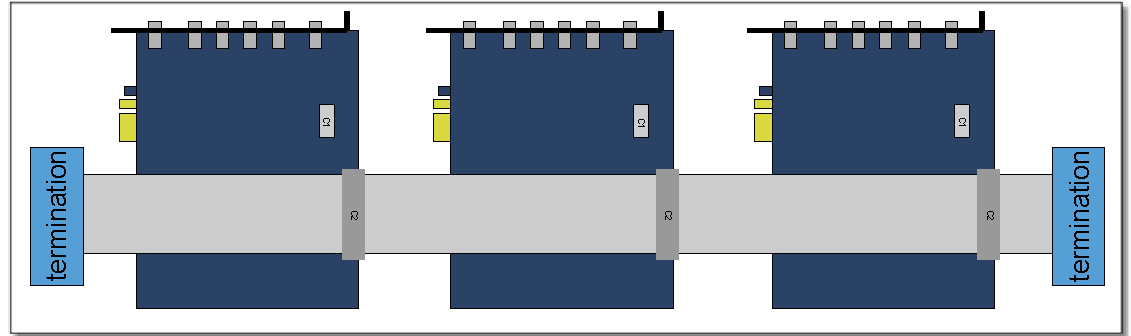
\includegraphics[width=\textwidth]{figures/Ndigo_Intercon.pdf}
    \caption{If several Ndigo boards are connected to work in sync, the boards must be connected using a ribbon cable as bus for synchronization and trigger signals. At both ends of the cable, proper termination is required.}
\end{figure*}
%
%
%
%
%
\clearpage
\section{Ndigo5G External Inputs and Connectors}
\subsection{Connectors}
%
The inputs of the Ndigo5G are located on the PCI bracket. Figure~\ref{fig:schematics} on page~\pageref{fig:schematics} shows the location of the 4 analog inputs A to D and the two digital inputs G (GATE) and T (Trigger). Furthermore, two board interconnection connectors can be found at the top edge of the Ndigo5G, as displayed in  Figure \ref{fig:schematics} on page \pageref{fig:schematics}. Connector C1 is used for a board-to-board connection (e.g., to link a HPTDC8-PCI and a Ndigo5G via a Ndigo Extension board, see chapter \ref{cp:extcard}). Connector C2 is used as a bus interface between multiple Ndigo boards distributing clock, trigger and sync signals. Proper termination must be placed at both ends of the bus interconnection ribbon cable.
%
\begin{figure*}[hb]
    \centering
    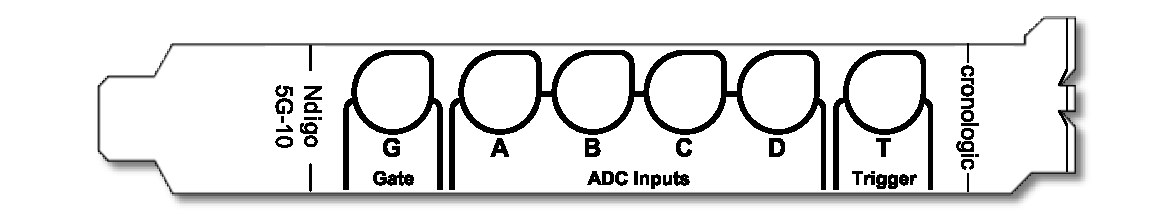
\includegraphics[width=0.6\textwidth]{figures/Ndigo-Slotblende.pdf}
    \caption{Input connectors of an Ndigo5G located on the PCI bracket.}
\end{figure*}
%
\begin{figure*}[ht]
    \centering
    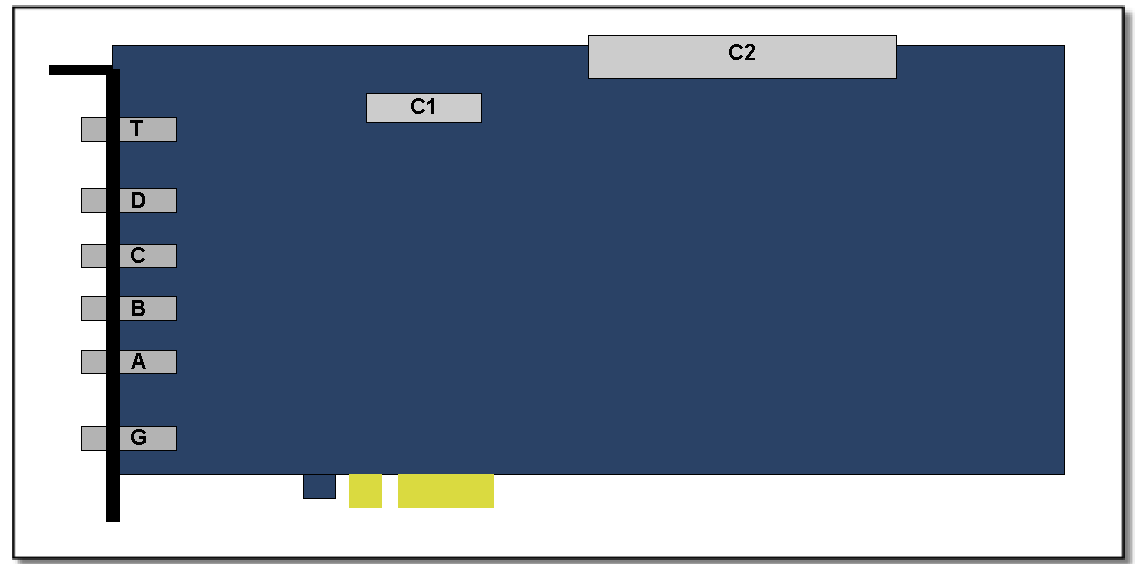
\includegraphics[width=0.7\textwidth]{figures/Ndigo_schematic.pdf}
    \caption{Schematics of an Ndigo5G board showing inter-board connectors C1 and C2.\label{fig:schematics}}
\end{figure*}
%
%
%
\subsection{Analog Inputs}
%
\begin{figure*}[ht]
    \centering
    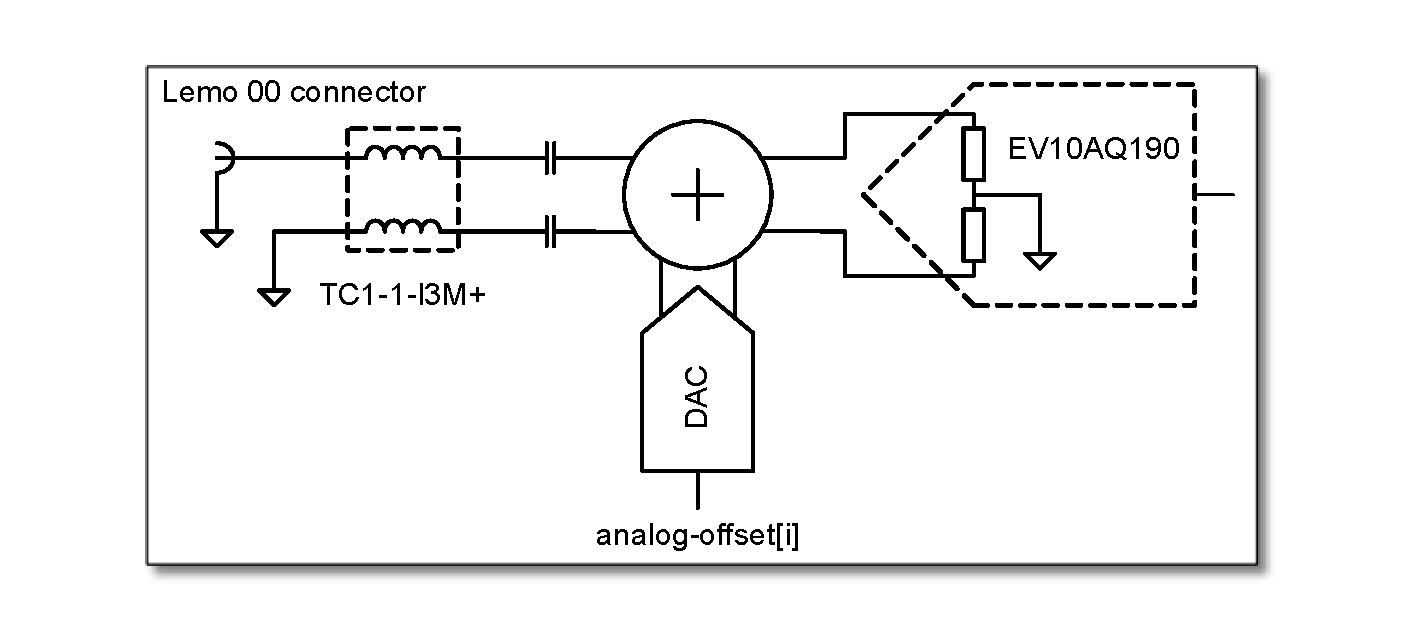
\includegraphics[width=0.8\textwidth]{figures/InputCircuit.pdf}
    \caption{Input circuit for each of the four analog channels.}
\end{figure*}
%
The analog inputs of the ADC are single ended LEMO00 coax connectors. The inputs have a $50\Omega$ impedance and are AC coupled. The inputs are converted to a differential signal using a balun.
%
%
%
\subsubsection{Analog Offsets}
%
\begin{figure*}[ht]
    \centering
    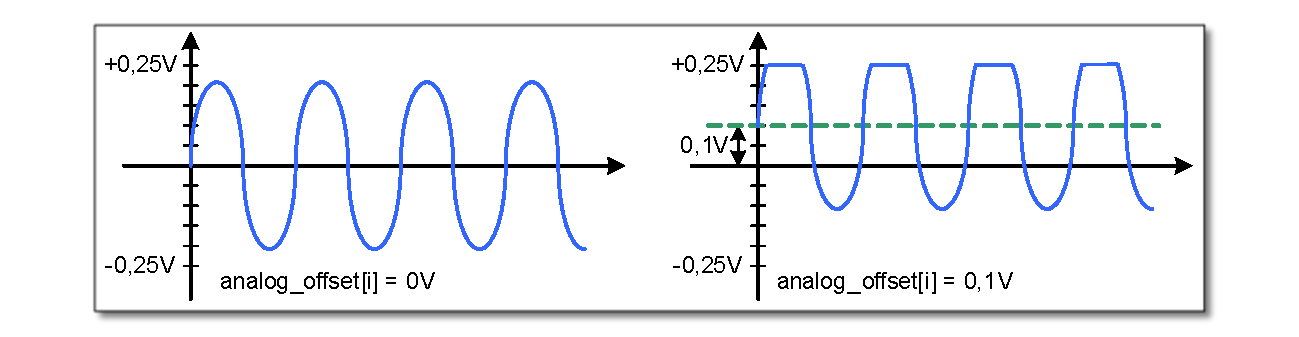
\includegraphics[width=\textwidth]{figures/AnalogOffset_Sine.pdf}
    \caption{Users can add analog offset to the input before sampling}
\end{figure*}
%
AC coupling removes the common mode voltage from the input signal. Users can move the common mode voltage to a value of their choice using the analog\tu offset parameter of each channel before sampling.\par
%
\begin{figure*}[!ht]
    \centering
    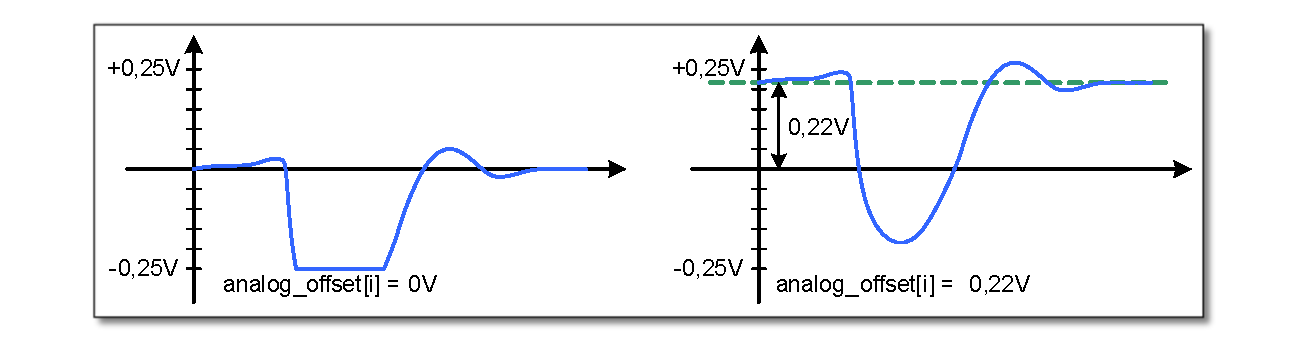
\includegraphics[width=\textwidth]{figures/AnalogOffset_Pulse.pdf}
    \caption{Asymmetric signal shifted to increase dynamic range\label{fig:shiftInput}}
\end{figure*}
%
This feature is useful for highly asymmetric signals, such as pulses from TOF spectrometers or LIDAR systems. Without analog offset compensation, the pulses would begin in the middle of the ADC range, effectively cutting the dynamic range in half (see Figure \ref{fig:shiftInput}). By shifting the DC baseline to one end of the ADC range, the input range can be used fully, providing the maximum dynamic range. The analog offset can be set between $\pm 0,25V$.
%
%
%
\subsection{Digital Inputs}
%
There are two digital inputs on the front slot cover called Trigger and Gate.\par
Both inputs provide a digital input signal routed to the trigger matrix. These signals can be used to trigger any of the trigger state machines and gating blocks. The inputs are AC coupled. DC offset is configurable via the \textsf{dc\tu offset} parameter in the configurations structure to support positive and negative input pulses. \textsf{dc\tu offset[1]} is the offset for the Trigger input and \textsf{dc\tu offset[0]} is the offset for the GATE input.\par
The configuration is set via the structures \textsf{trigger\allowbreak [NDIGO\tu TRIGGER\tu TRIGGER]} for the Trigger input and \textsf{trigger[NDIGO\tu TRIGGER\tu GATE]} for the GATE input. The input circuit is shown in Figure \ref{fig:DigitalInput} on page \pageref{fig:DigitalInput}.
%
%
%
\subsubsection{TDC on Trigger Input}
%
There is a TDC connected to the Trigger input. When used with the TDC, the Trigger input supports negative pulses only . The TDC creates packets of type 8. These packets first contain a coarse timestamp and a payload that can be used to calculate the trigger position with higher precision. The function \textsf{ndigo\tu process\tu tdc\tu packet()} can be used to replace the coarse timestamp with the precise timestamp. This function is described in section \ref{cp:readout} on page \pageref{cp:readout}.
TDC pulses must have a minimum duration of 3.3ns. The dead-time of the TDC is 32ns.

\textsf{NDIGO\tu TRIGGER\tu TDC} is an alias for \textsf{NDIGO\tu TRIGGER\tu TRIGGER}.
%
%
%
%
%
\section{Extension Card\label{cp:extcard}}

The Ndigo Extension card provides additional inputs or outputs to the FPGA. It is connected to the Samtec QSS-025 connector on an Ndigo5G by a Samtec SQCD cable assembly.\par
The Ndigo Extension Card provides up to ten single ended LEMO00 connectors. The circuit connecting to each of these circuits can be chosen to provide inputs or outputs. These can be AC or DC coupled. AC coupled inputs support NIM signaling. The signals connect to 2.5V IO Pins of the Xilinx Virtex-5 FPGA.\par
The current firmware revision provides the following signal connections. The HPTDC clocks are $\SI{5}{\giga\hertz} / 128 = \SI{39.0625}{\mega\hertz}$\par

\begin{small}
\begin{center}
\begin{tabular}{|c|c|c|c|c|}
    \hline
    Connector & QSS Pin & FPGA Pin & Direction & Signal\\
    \hline\hline
    LEMO00: CH0 & 22 & AD9 & Input & Ndigo Extension digital channel 0\\\hline
    LEMO00: CH1 & 18 & AE10 & Input & Ndigo Extension digital channel 1\\\hline
    LEMO00: CH2 & 14 & D10 & - & not connected\\\hline
    LEMO00: CH3 & 10 & AF9 & Output & \SI{39.0625}{\mega\hertz} clock for HPTDC\\\hline
    LEMO00: CH4 & 6 & AD11 & Output & 39.0625 MHz clock for HPTDC\\\hline
    LEMO00: CH5 & 5 & AE7 & Output & 39.0625 MHz clock for HPTDC\\\hline
    LEMO00: CH6 & 9 & AF7 & Output & 39.0625 MHz clock for HPTDC\\\hline
    LEMO00: CH7 & 13 & D9 & - & not connected\\\hline
    LEMO00: CH8 & 17 & V9 & Input & Ndigo Extension digital channel 2\\\hline
    LEMO00: CH9 & 21 & W9 & Input & Ndigo Extension digital channel 3\\\hline
    SYNC1: Sync-TDC8 & 26 & F9 & - & not connected\\\hline
    SYNC1: Sync-HPTDC & 44 & AA7 & Output & Sync for HPTDC\\\hline
\end{tabular}
\end{center}
\end{small}

The 4 digital inputs are routed to the bus inputs of the trigger matrix to be used for triggering. The routing can be configured to either OR-ing the sync bus and extension channels or use the extension channels exclusively.

\begin{center}
\begin{tabular}{|c|c|c|c|}
    \hline
    Connector & Extension Card & Trigger matrix input  & Trigger matrix input\\
    & Digital Channel & ignore\tu cable = 0 & ignore\tu cable = 1\\
    \hline\hline
    LEMO00: CH0 & 0 & BUS0 = EXT0 \textbar\ Sync Cable 0 & BUS0 = EXT0\\\hline
    LEMO00: CH1 & 1 & BUS1 = EXT1 \textbar\ Sync Cable 1 & BUS1 = EXT1\\\hline
    LEMO00: CH8 & 2 & BUS2 = EXT2 \textbar\ Sync Cable 2 & BUS2 = EXT2\\\hline
    LEMO00: CH9 & 3 & BUS3 = EXT3 \textbar\ Sync Cable 3 & BUS3 = EXT3\\\hline
\end{tabular}
\end{center}
%
%
%
%
%
\section{Ndigo5G Functionality}
\subsection{ADC Modes}

Depending on board configuration, the analog input signal is quantized to 8 or 10 bits. However, the board always scales and offsets the data to 16-bit signed data centered around 0.\par
Data processing such as trigger detection or packet building are always performed on 3.2ns intervals. Depending on the ADC mode, this interval may contain 4, 8 or 16 samples.\par
The board supports using one, two or four channels:

\subsubsection{1-Channel-Modes A, B, C and D}

In these modes, only a single channel is used. The analog signal on that channel is digitized at 5Gsps. Packet size is always a multiple of 16 samples per 3.2ns. See Figure \ref{fig:1ChannelMode} on page \pageref{fig:1ChannelMode} and Figure \ref{fig:1ChannelTriggering} on page \pageref{fig:1ChannelTriggering}.

\subsubsection{2-Channel-Modes AC, BC, AD and BD}

In these modes, two channels are used simultaneously. The analog signals on these channels are digitized at 2.5Gsps each. Packet size is always a multiple of 8 samples per 3.2ns. See Figure \ref{fig:2ChannelMode} on page \pageref{fig:2ChannelMode} and Figure \ref{fig:2ChannelTriggering} on page \pageref{fig:2ChannelTriggering}.

\subsubsection{4-Channel-Mode ABCD}

In this mode, all four channels are digitized independently at 1.25Gsps each. The packet size is always a multiple of 4 samples per 3.2ns. See Figure \ref{fig:4ChannelMode} on page \pageref{fig:4ChannelMode} and Figure \ref{fig:4ChannelTriggering} on page \pageref{fig:4ChannelTriggering}.

\subsubsection{Multiple Sampling Modes AAAA, BBBB, CCCC and DDDD}

In these modes, only one analog input channel is used, but the channel is sampled independently and simultaneously by four ADCs at 1.25Gsps. The board creates four independent streams with 4 samples each per 3.2ns.\par
Using the same trigger setting on all ADCs, can be used to reduce noise by averaging the four channels. To deal with complex triggering conditions, different trigger settings on each of the ADCs can be used.\par
The Ndigo5G provides 4 ADCs sampling at 1.25Gsps each. Higher speed modes are implemented by interleaving two or four of these ADCs.\par
During interleaving, the Ndigo5G firmware reorders and groups the data into a linear sample stream. The process is fully transparent. For users, the only difference is that a 3.2ns cycle can contain 4, 8 or 16 samples, depending on mode.

\begin{figure}
    \centering
    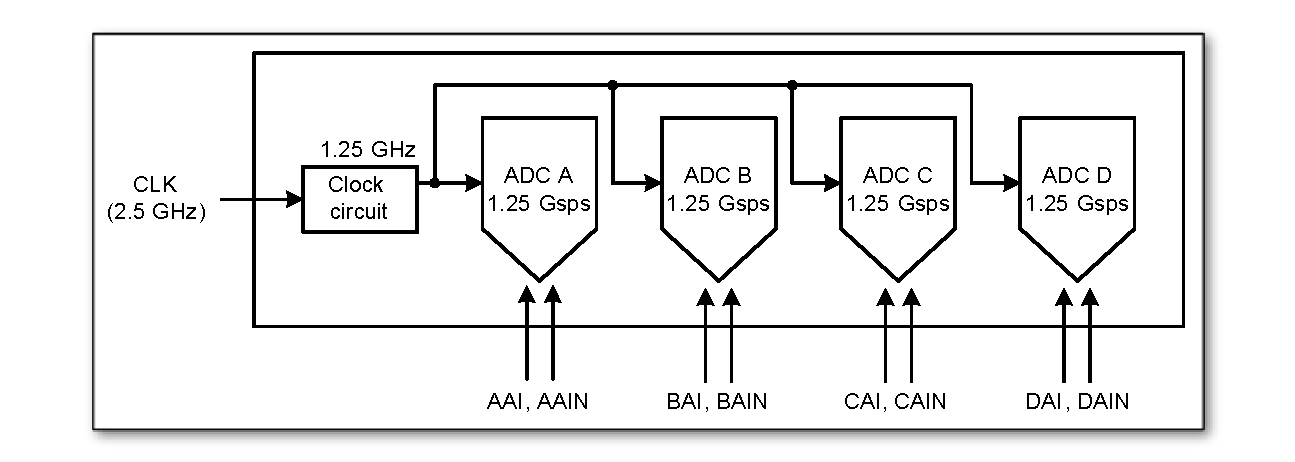
\includegraphics[width=\textwidth]{figures/4ChannelMode.pdf}
    \caption{ADCs in 4-channel-mode ABCD at 1.25Gsps.\label{fig:4ChannelMode}}
\end{figure}

\begin{figure}
    \centering
    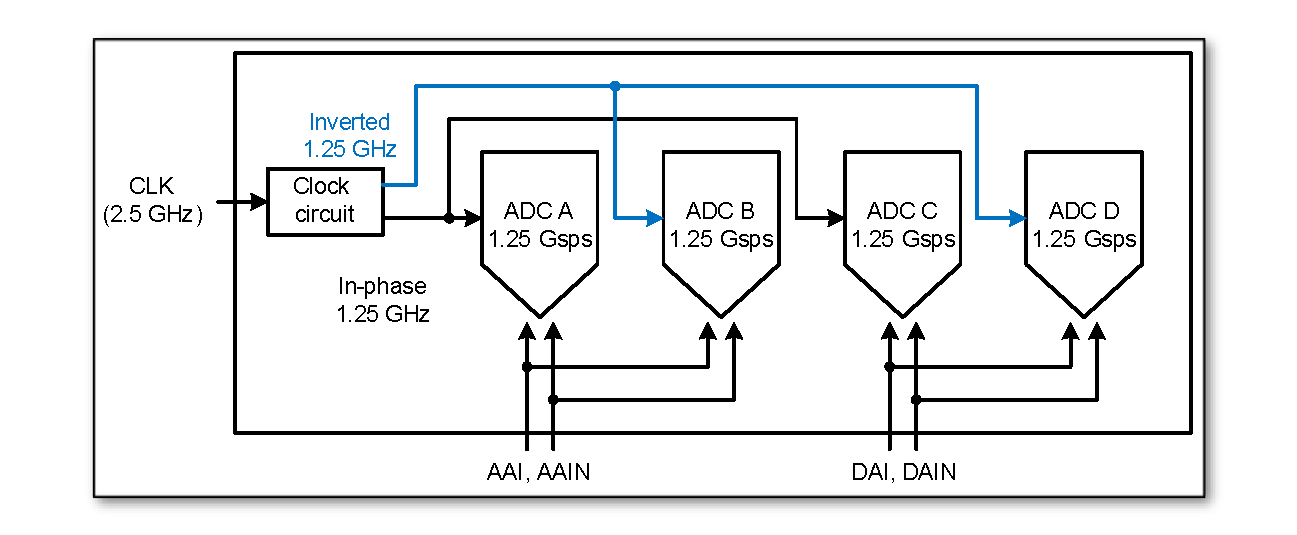
\includegraphics[width=\textwidth]{figures/2ChannelMode.pdf}
    \caption{ADCs in 2-channel-mode AD, interleaved for 2.5Gsps.\label{fig:2ChannelMode}}
\end{figure}

\begin{figure}
    \centering
    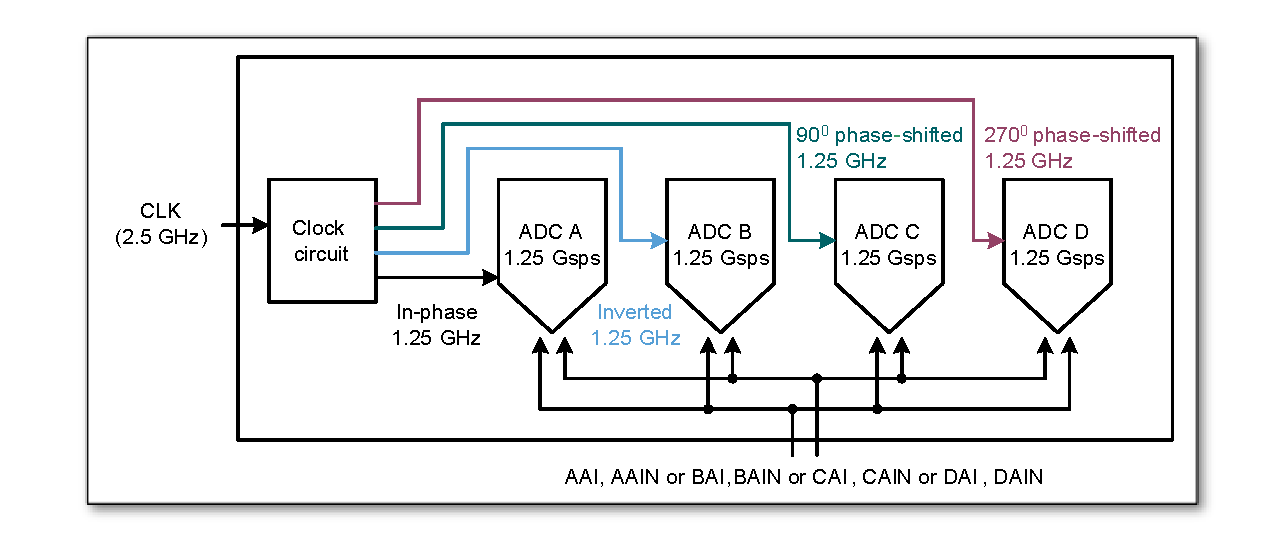
\includegraphics[width=\textwidth]{figures/1ChannelMode.pdf}
    \caption{ADCs in 1-channel-mode A, B, C or D interleaved for 5Gsps.\label{fig:1ChannelMode}}
\end{figure}

\clearpage
\subsection{Zero Suppression}

One of Ndigo5G's key features is on-board zero suppression to reduce PCIe bus load. Only data that passes specifications predefined by the user is transmitted. This guide refers to transmitted waveform data as ``packets.'' A packet contains the waveform data and a timestamp giving the absolute time (i.e., the time since start of data acquisition) of the packet's last sample.\par Figure \ref{fig:ZeroSupp} shows a simple example: Data is written to the PC only if values exceed a specified threshold. Expanding on that, Ndigo5G's zero suppression can be used to realize much more complex scenarios.

\begin{figure*}[hb]
    \centering
    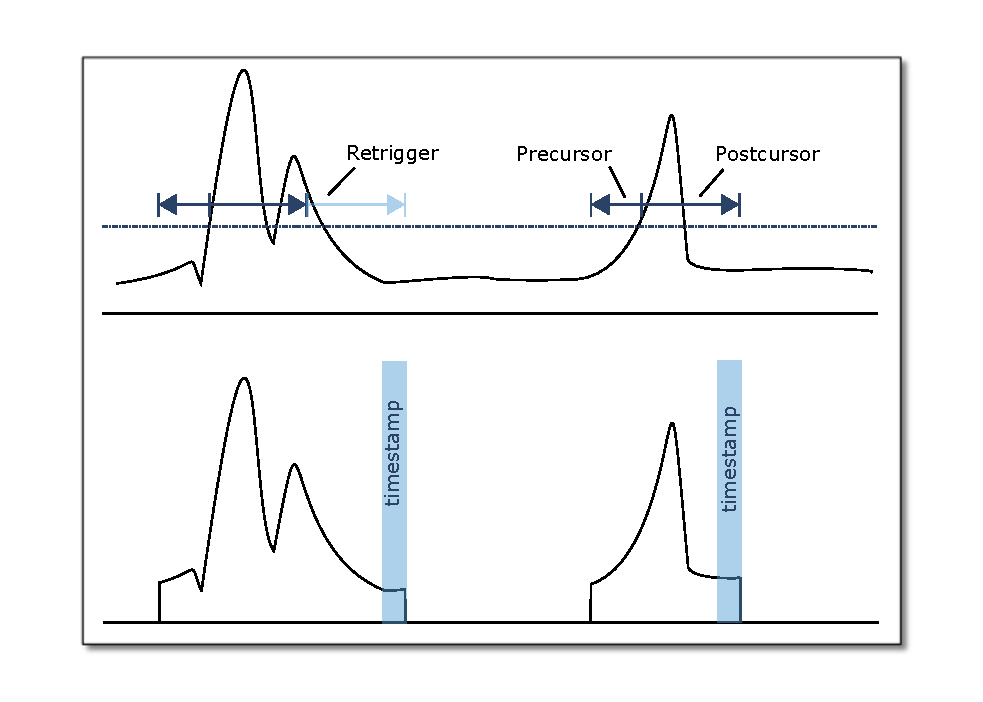
\includegraphics[width=0.8\textwidth]{figures/ZeroSupp.pdf}
    \caption{Simple zero suppression: Only data with values above a threshold are written to the PC.\label{fig:ZeroSupp}}
\end{figure*}

\subsection{Trigger Blocks}

Ndigo5G-10 and Ndigo5G-8 record analog waveforms using zero suppression. Whenever a relevant waveform is detected, data is written to an internal FIFO memory. Each ADC channel has one trigger block determining whether data is written to the FIFO. The parameters are set in  Structure \textsf{ndigo\tu trigger\tu block}(See chapter \ref{cp:triggerblock} on page \pageref{cp:triggerblock}).\par

Each trigger block consists of two independent units that check the incoming raw data stream for trigger conditions (Fig. \ref{fig:ZeroSupp} on page \pageref{fig:ZeroSupp}). Users can specify a threshold and can choose whether triggering is used whenever incoming data is below or above the threshold (level triggering) or only if data exceeds the threshold (edge triggering).\par

A gate length can be set to extend the trigger window by multiples of 3.2ns. Furthermore, if users choose precursor values $> 0$, the trigger unit will start writing data to the FIFO $\text{precursor}\cdot 3.2ns$ before the trigger event.\par

When using edge triggering, all packets have the same length (Figure \ref{fig:edge-trigger} on page \pageref{fig:edge-trigger}): $\text{precursor}+\text{length}+1$ cycles of 3.2ns. For level triggering, packet length is data dependent (Figure \ref{fig:level-trigger} on page \pageref{fig:level-trigger}).\par

Please note that triggering is not accurate to sample. For each 3.2ns clock cycle, it is determined whether on any sample during that clock cycle a trigger condition is met. The clock cycle is then selected as the trigger point. As a result, the trigger sample can be anywhere within a range of up to 16 samples in single channel mode (Figure \ref{fig:1ChannelTriggering} on page \pageref{fig:1ChannelTriggering}) at 16 samples per 3.2ns.\par

If re-triggering is active, the current trigger window is extended if a trigger event is detected inside the window.\par

A trigger block can use several input sources:

\begin{itemize}
    \item the 8 trigger decision units of all four ADC channels (Figure \ref{fig:analog-trigger} on page \pageref{fig:analog-trigger})
    \item the GATE input (Figure \ref{fig:DigitalInput} on page \pageref{fig:DigitalInput})
    \item the Trigger or TDC input,  (Figure \ref{fig:DigitalInput} on page \pageref{fig:DigitalInput})
    \item a function trigger providing random or periodic triggering (Section \ref{cp:AutoTriggeringFunctionGenerator} on page \pageref{cp:AutoTriggeringFunctionGenerator})
    \item triggers originating from other cards connected with the sync cable or from the Ndigo Extension card (BUS0, BUS1, BUS2, BUS3)
    \item A second set of trigger units with names ending in \textsf{\tu pe} for the digital inputs Trigger, GATE, BUS0, BUS1, BUS2, and BUS3 configured for positive edge triggering. Together with the regular trigger units on these inputs, both edges of a pulse can be used in the trigger logic. This set of triggers is not available as inputs for the gate blocks.
\end{itemize}

Trigger inputs from the above sources can be concatenated using logical ``OR'' (Figure \ref{fig:triggermatrix} on page \pageref{fig:triggermatrix}) by setting the appropriate bits in the trigger blocks source mask.\par

Triggers can be fed into the gate blocks described on page \pageref{fig:GatingBlock} (Figure \ref{fig:GatingBlock}). Gate blocks can be used to block writing data to the FIFO. That way, only zero suppressed data occurring when the selected gate is active is transmitted. This procedure reduces PCIe bus load even further (Figure \ref{fig:GatingBlock}).

\begin{figure*}[ht]
    \centering
    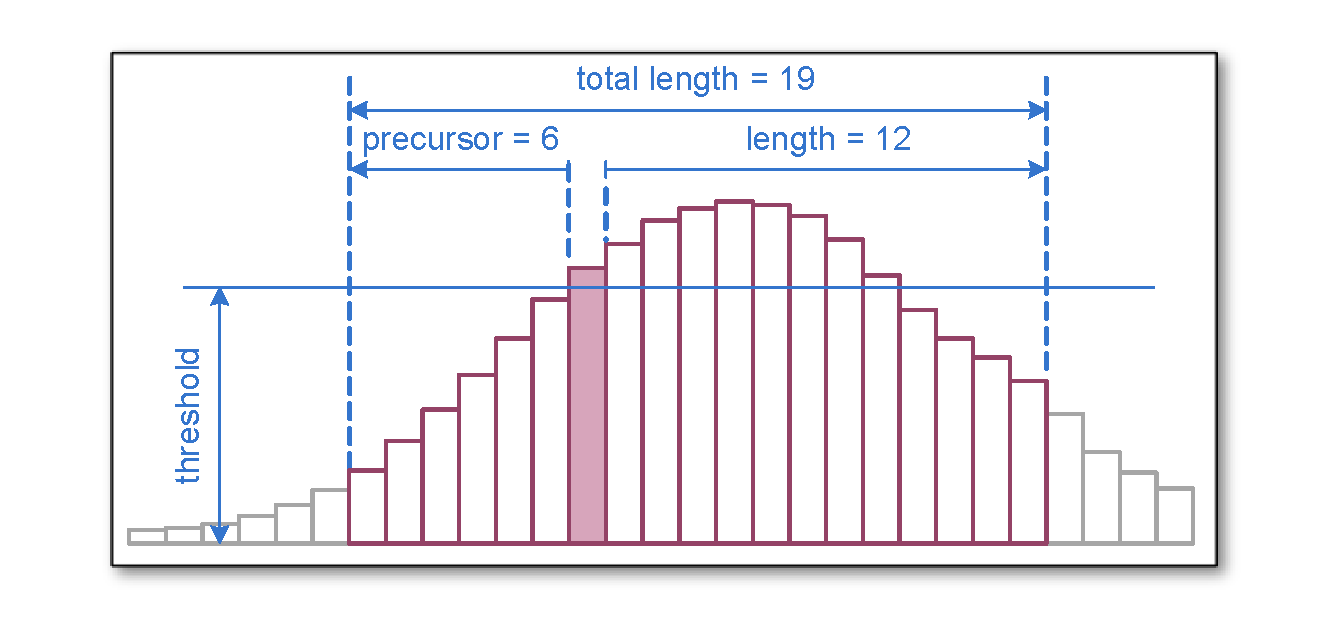
\includegraphics[width=0.8\textwidth]{figures/edge-trigger.pdf}
    \caption{Parameters for edge triggering\label{fig:edge-trigger}}
\end{figure*}

\begin{figure*}[hb]
    \centering
    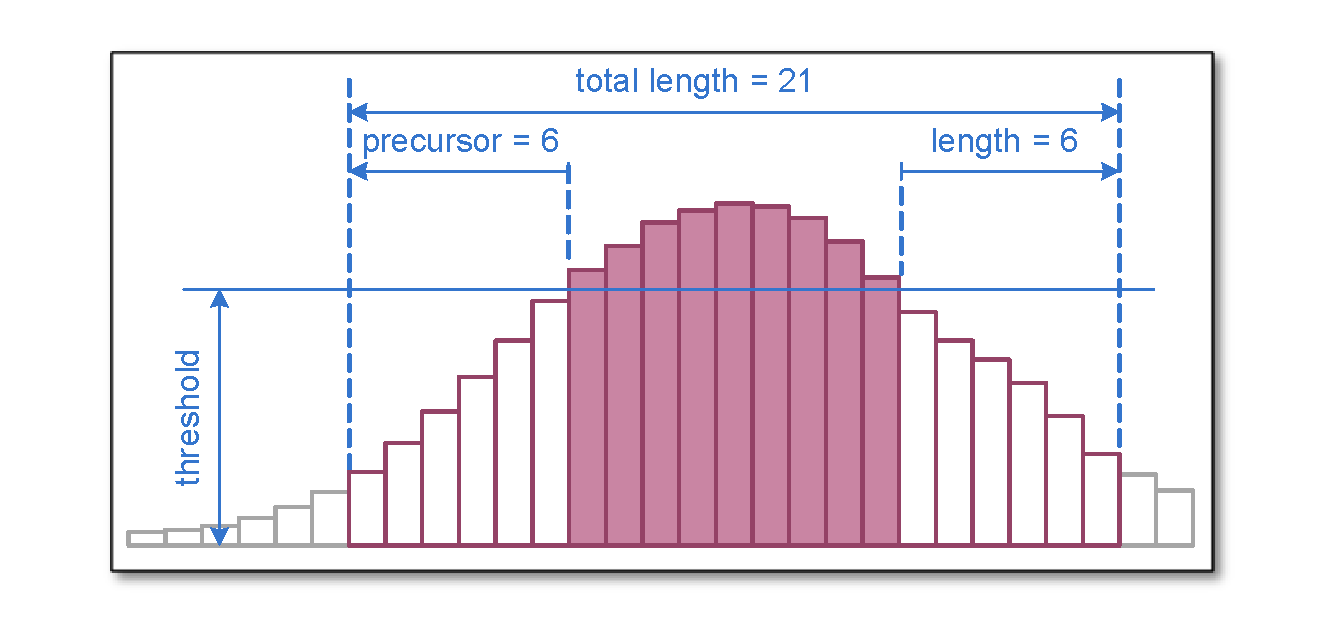
\includegraphics[width=0.8\textwidth]{figures/level-trigger.pdf}
    \caption{Parameters for level triggering\label{fig:level-trigger}}
\end{figure*}

\begin{figure*}[ht]
    \centering
    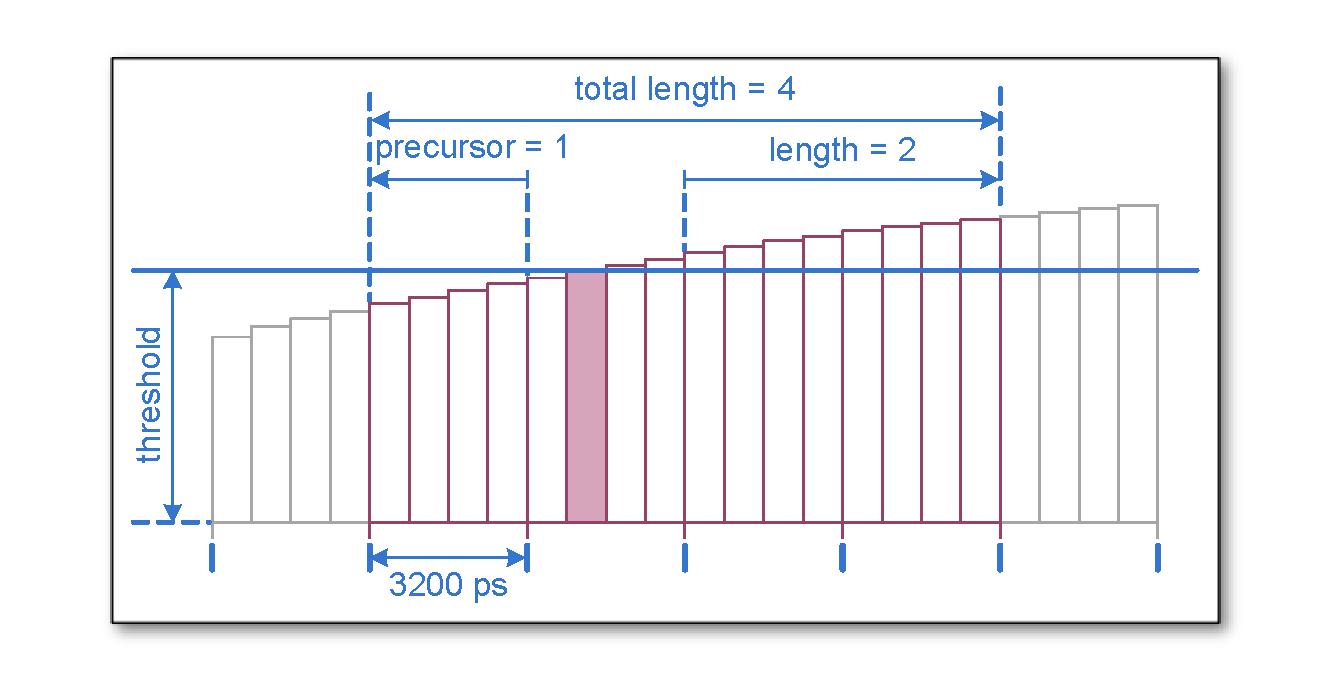
\includegraphics[width=0.8\textwidth]{figures/4ChannelTriggering.pdf}
    \caption{Triggering in 4-channel mode at 4 samples per clock cycle.\label{fig:4ChannelTriggering}}
\end{figure*}

\begin{figure*}[hb]
    \centering
    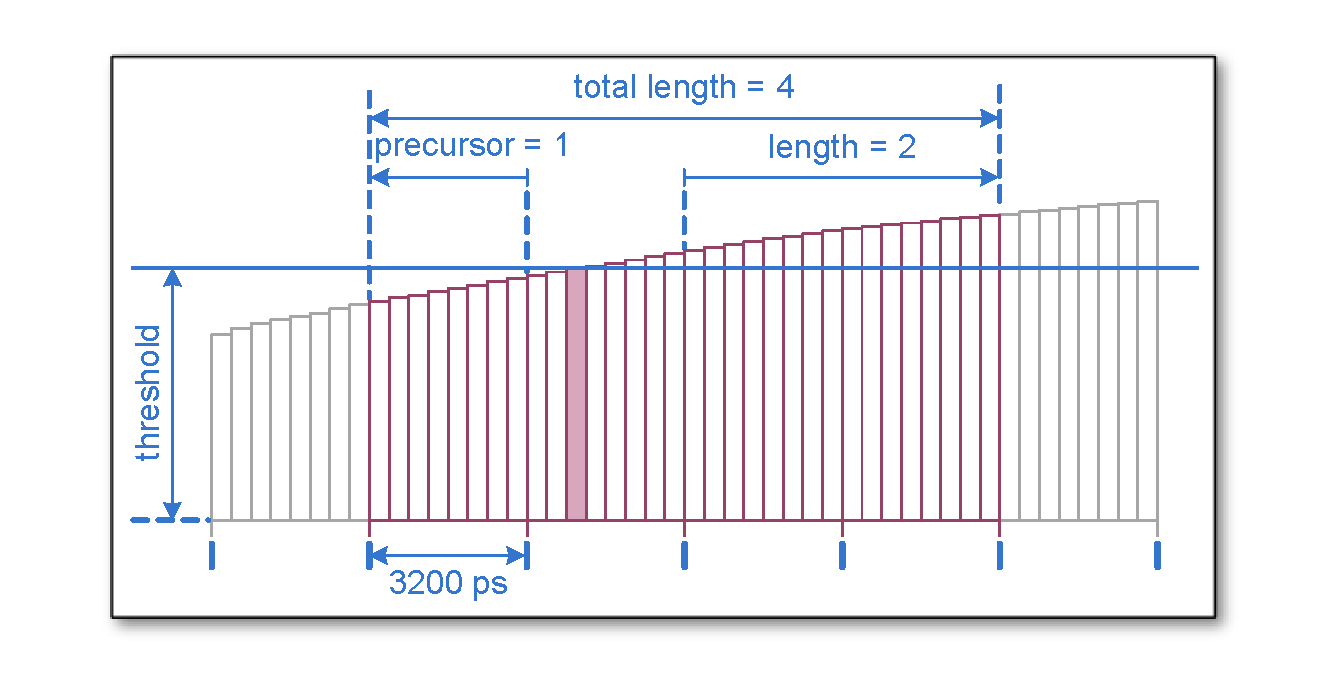
\includegraphics[width=0.8\textwidth]{figures/2ChannelTriggering.pdf}
    \caption{Triggering in 2-channel mode at 8 samples per clock cycle.\label{fig:2ChannelTriggering}}
\end{figure*}

\begin{figure*}[ht]
    \centering
    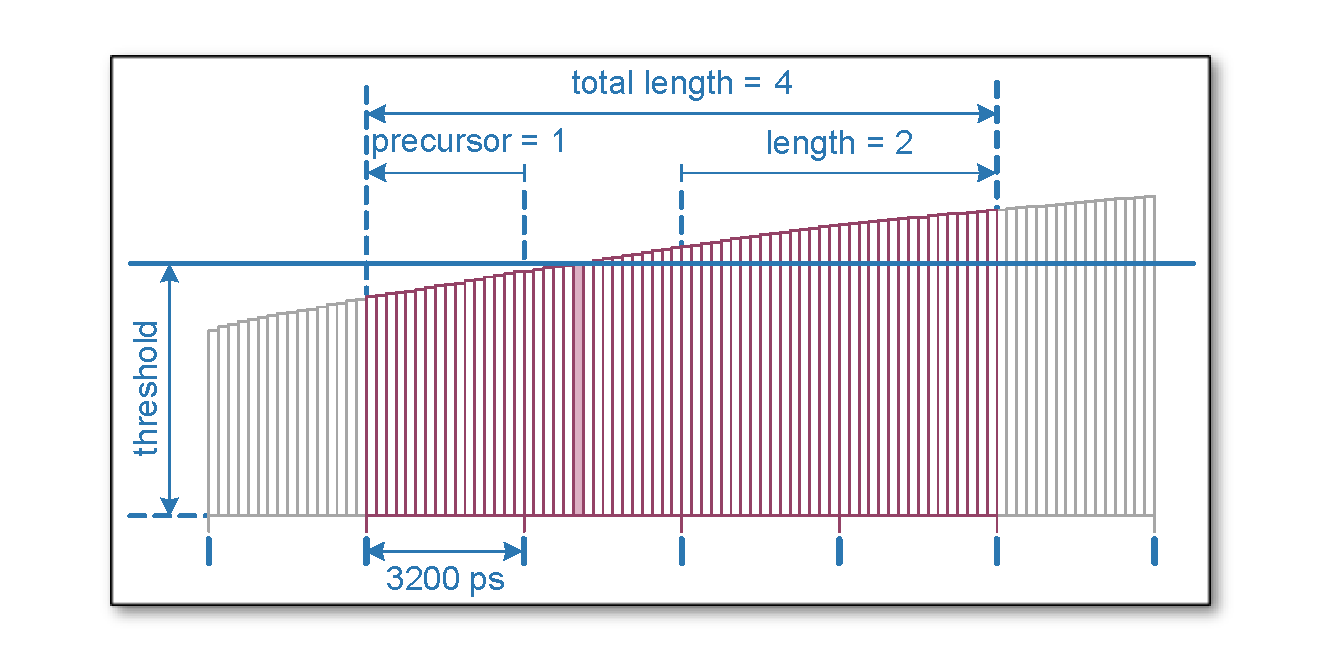
\includegraphics[width=0.8\textwidth]{figures/1ChannelTriggering.pdf}
    \caption{Triggering in 1-channel mode at 16 samples per clock cycle.\label{fig:1ChannelTriggering}}
\end{figure*}

\begin{figure*}[hb]
    \centering
    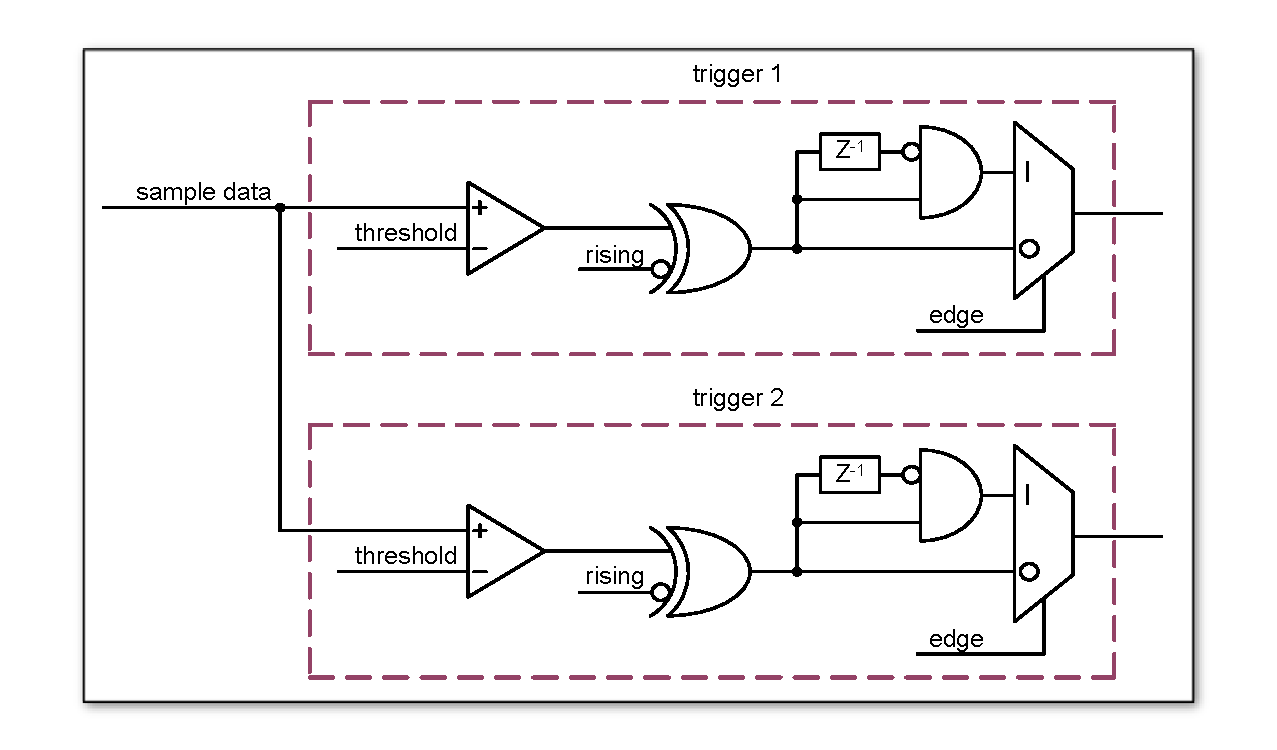
\includegraphics[width=0.8\textwidth]{figures/analog-trigger.pdf}
    \caption{From the ADC inputs, a trigger unit creates an input flag for the trigger matrix. Each digitizer channel (A, B, C, D) has two trigger units.\label{fig:analog-trigger}}
\end{figure*}

\begin{figure*}[ht]
    \centering
    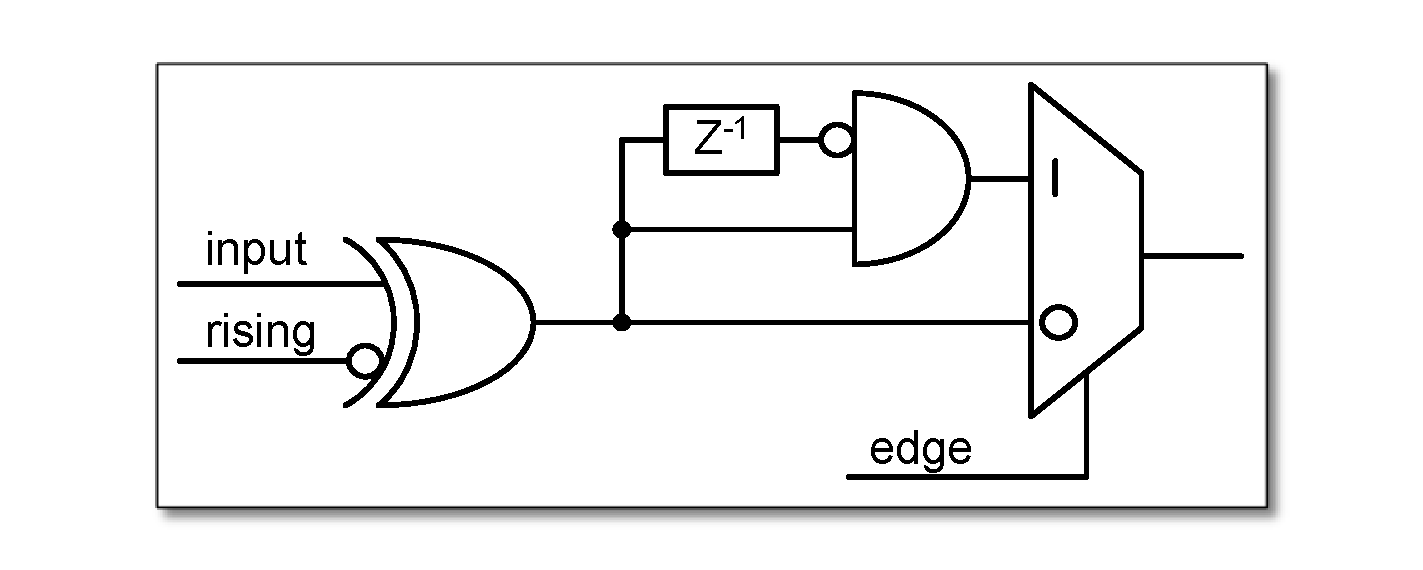
\includegraphics[width=0.5\textwidth]{figures/DigitalInput.pdf}
    \caption{The digital inputs Trigger, GATE, BUS0, BUS1, BUS2 and BUS3 have simpler trigger units.\label{fig:DigitalInput}}
\end{figure*}

\begin{figure*}
    \centering
    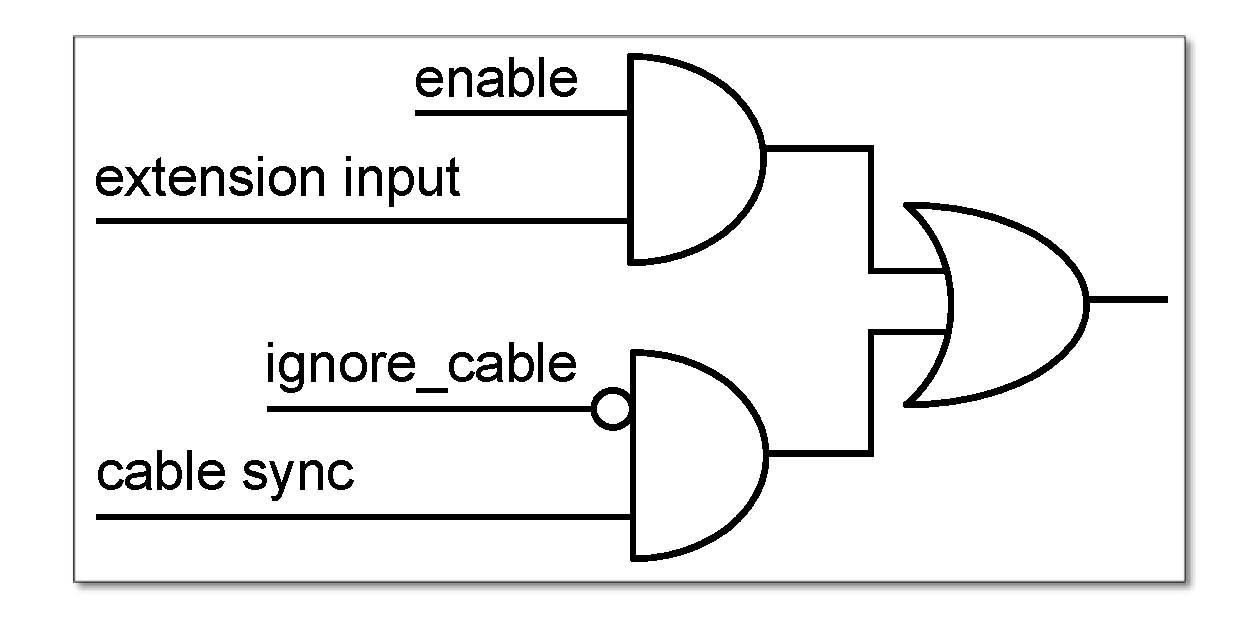
\includegraphics[width=0.5\textwidth]{figures/ExtensionBlock.pdf}
    \caption{\label{fig:ExtensionBlock} The extension block combines signals from the optional extension board and the sync cable.}
\end{figure*}

\begin{figure*}
    \centering
    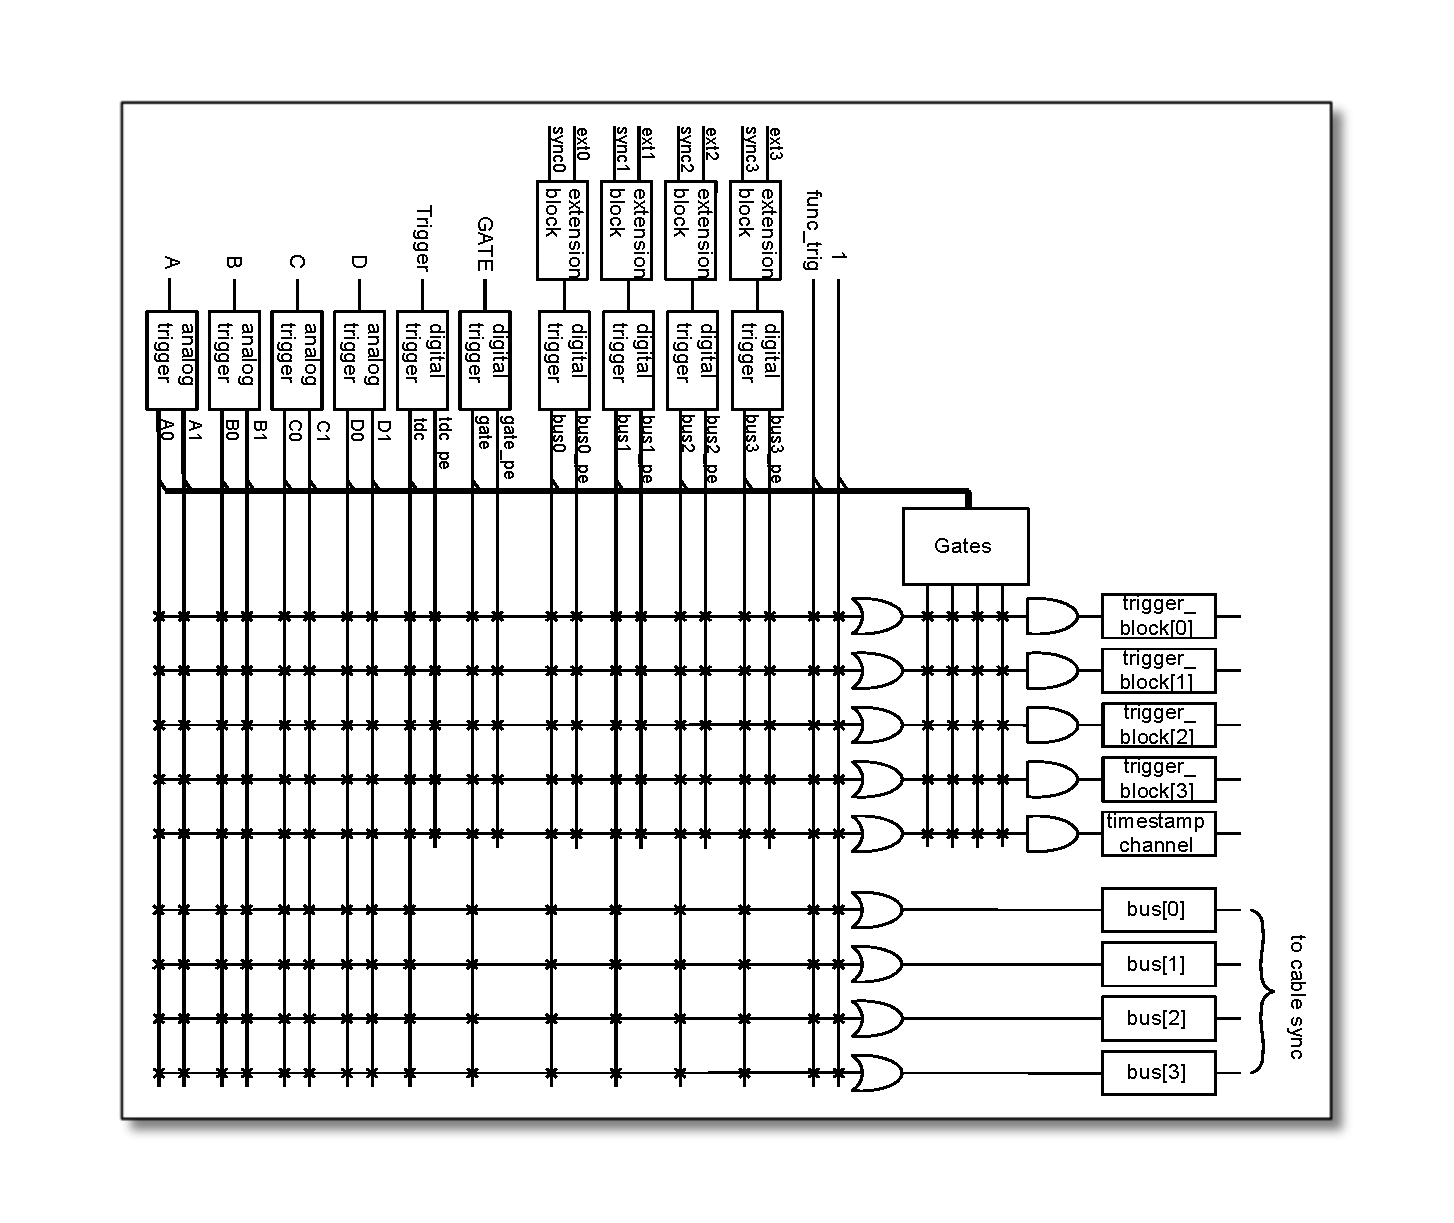
\includegraphics[width=\textwidth]{figures/triggermatrix.pdf}
    \caption{Trigger Matrix: The trigger signals of each ADC channel, the Trigger input, the GATE input or the sync cable can be combined to create a trigger input for each trigger block.  The four gate signals can be used to suppress triggers during certain time frames.\label{fig:triggermatrix}}
\end{figure*}

\subsection{Gating Blocks}

        \begin{figure*}[ht]
            \begin{center}
                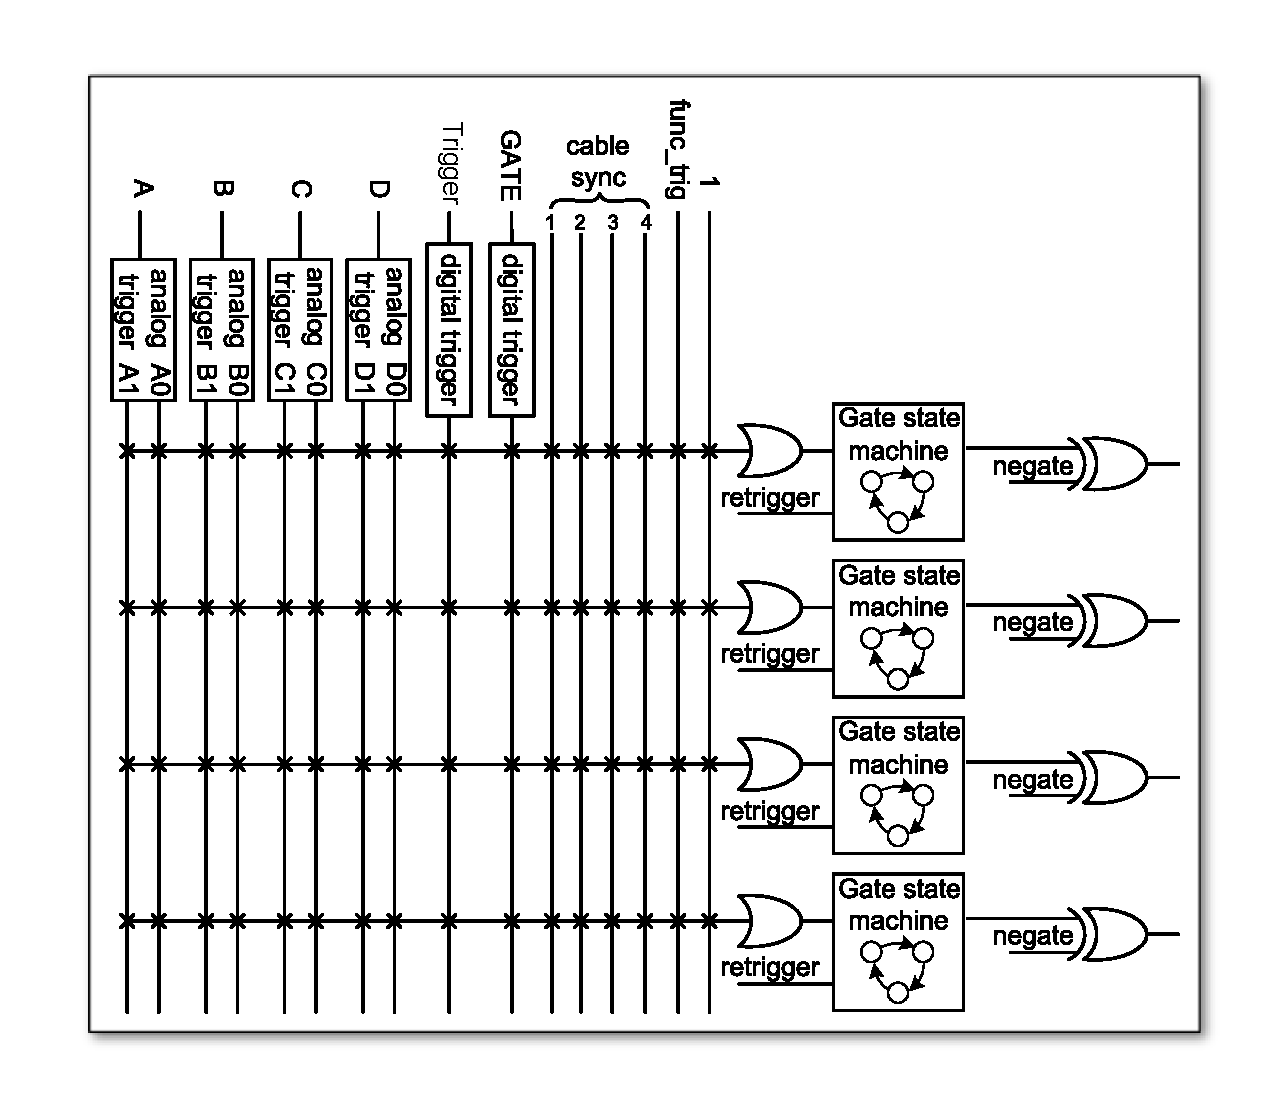
\includegraphics[width=0.8\textwidth]{figures/GatingBlocks.pdf}
                \caption{\label{fig:GatingBlock} Gating Blocks: Each gating block can use an arbitrary combination of inputs to trigger its state machine. The outputs can be individually inverted and routed to the AND-gate feeding the trigger blocks.}
            \end{center}
        \end{figure*}

        To decrease the amount of data transmitted to the PC, Ndigo5G includes 4 independent gate and delay units. A gate and delay unit creates a gate window starting at a specified time after a trigger, closing the window at gate stop. Both timing values — gate start and gate stop — must be set as multiples of 3.2ns.\par

        Trigger blocks can use the gate signal to suppress data acquisition: Only data that fulfills zero suppression specifications occurring in an active gate window is written to the PC.\par
        As input, any trigger from the 4 trigger blocks, the GATE and Trigger inputs, a trigger from a connected board and the function generator can be used.\par

        The re-trigger feature will create a new gate if a trigger occurs during an active gate window. The gate signal can be inverted, causing an active gate to close for a time defined by the user.\par

        The parameters of a gating block are set in Structure \textsf{ndigo\tu gating\tu block} described on page \pageref{cp:gatingblock}.\par

        Figure \ref{fig:GateUDelay} shows the functionality of the gate timing and delay unit. Active gate time is marked in green.

        \begin{figure*}[ht]
            \begin{center}
                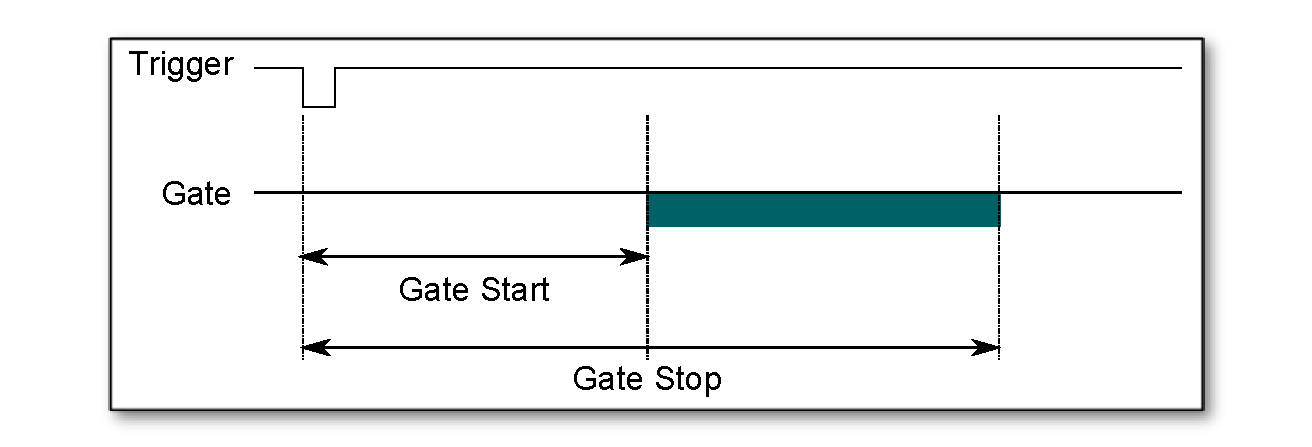
\includegraphics[width=0.8\textwidth]{figures/GateUDelay.pdf}
                \caption{\label{fig:GateUDelay} Gate and delay functionality: When a trigger occurs, the gate opens after a set period of time (``gate start'') and closes when it reaches ``gate stop''.}
            \end{center}
        \end{figure*}

        \subsubsection{Gating Example 1: Suppression of Noise After Starting an Acquisition}

            In mass spectrometer and other experiments, noise while starting data acquisition can result in undesired trigger events for that time period. To prevent noise in the output data, a gating block could be used to suppress all triggers during start-up.\par

            The following example illustrates the use of a gating block to prevent noise: The GATE input transmits a pulse on each acquisition start. The trigger structure of the GATE input is used to select pulse polarity. Then, the GATE trigger is selected as gating block input and the gating block's start parameter is set to 0. The stop parameter is set to the desired length measured in 3.2ns clock cycle and negate is set to true. The gating block will now output a low pulse of the desired length whenever there is a pulse on the GATE input.\par

        Enabling this gating block as an AND input to the trigger block, for which noise shall be suppressed.

        \subsubsection{Gating Example 2: Delayed Trigger}

            To sample a short window at a specified time after a trigger event on a channel, the gating block can be used to create a delayed trigger. To do this, one of the triggers of the channel of interested is configured to the desired parameters by selecting the threshold, setting the edge polarity and enabling edge triggering.\par

            Instead of directly using this trigger as input to the trigger block's input matrix, the trigger is selected as an input to a gating block. The block is configured to $start = delay$ [in 3.2ns clock cycles] and $stop = start+1$, $negate = false$. This causes the gating block to produce a one clock cycle pulse on its output after the specified delay.\par

            To send this pulse to the trigger block, the gating block must be enabled in the trigger block's AND matrix and the ONE trigger source must be selected.

        \subsubsection{Gating Example 3: Dual Level Trigger}

            The gates provide AND connections between each other (see fig. \ref{fig:triggermatrix}) which can be used for example in a dual level trigger. For the acquisition of signal data with amplitudes between a lower and an upper bound, for example, two level triggers can be connected (see fig. \ref{fig:dualleveltrig}): a falling level trigger with an upper threshold and a rising level trigger with a lower threshold.\par
            Since the triggers are only connected by OR in the trigger-block logic (see fig. \ref{fig:triggermatrix}) they are assigned to one of the gates each and connected with AND via the gating block region of the trigger matrix (see fig. \ref{fig:triggermatrix} and \ref{fig:dualleveltriglogic}). Because of the dead times of the gates it is important to enable the re-triggering feature. Furthermore, a precursor of 2 clock cycles is needed, because the gates are delayed in relation to the ADC samples.\par
            \begin{figure*}[ht]
                \begin{center}
                    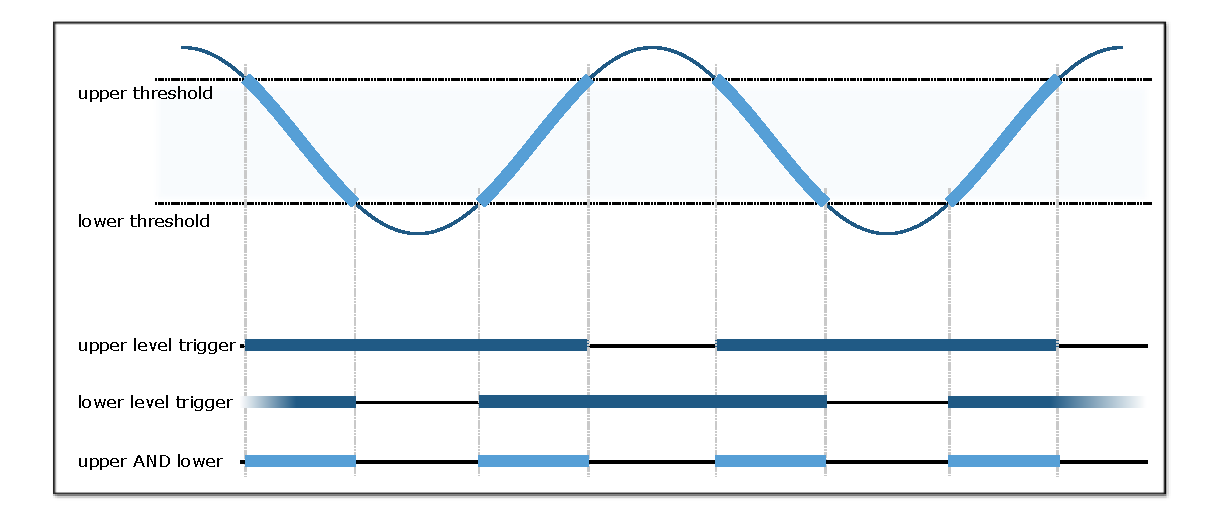
\includegraphics[width=\textwidth]{figures/dual_level_triggering.pdf}
                    \caption{\label{fig:dualleveltrig}Measuring data with amplitude between an upper and a lower threshold by means of two level triggers.}
                \end{center}
            \end{figure*}

            \begin{figure*}[ht]
                \begin{center}
                    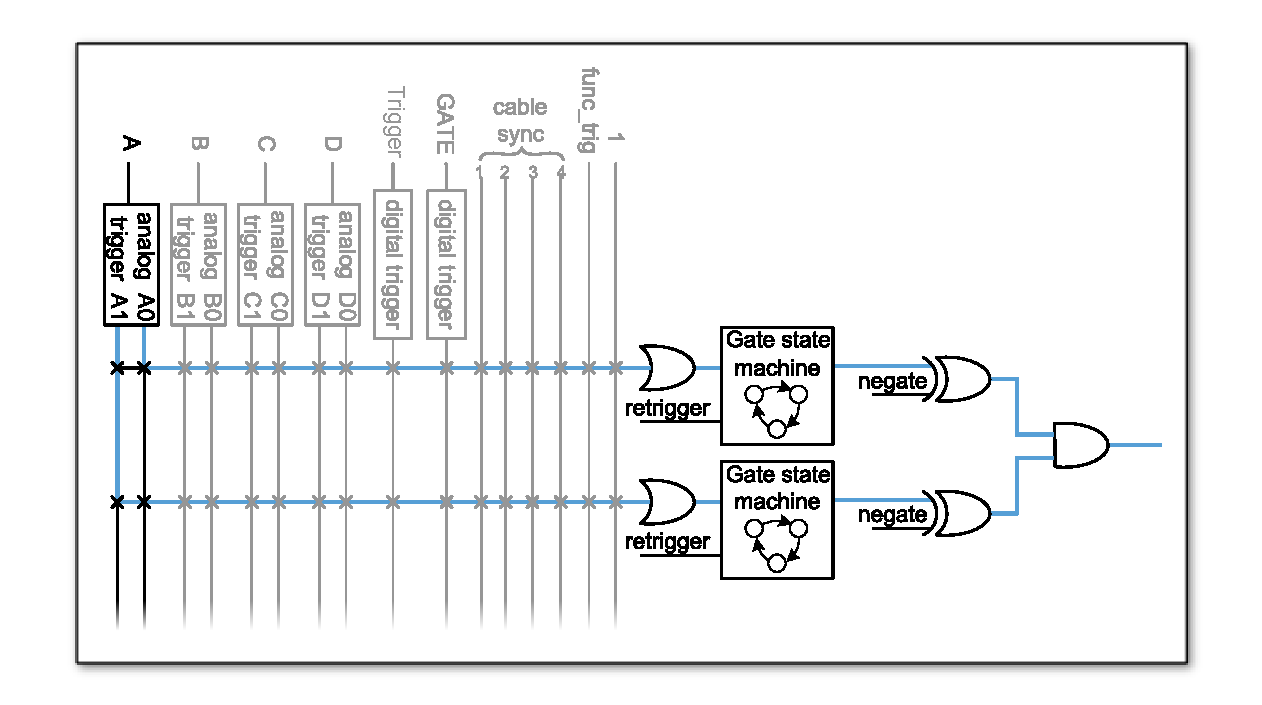
\includegraphics[width=\textwidth]{figures/dual-level-triggering_logic.pdf}
                    \caption{\label{fig:dualleveltriglogic}Gating block logic for the AND connection of two triggers.}
                \end{center}
            \end{figure*}

            Config settings can be found in the following code snippet.

\begin{lstlisting}[frame=tlrb]
    config.trigger_block[0].enabled = 1;
    config.trigger_block[0].precursor = 2;
    config.trigger_block[0].length = 0;
    config.trigger_block[0].sources = NDIGO_TRIGGER_SOURCE_ONE;
    config.trigger_block[0].gates = NDIGO_TRIGGER_GATE_0 | NDIGO_TRIGGER_GATE_1;
    config.gating_block[0].retrigger = 1;
    config.gating_block[0].stop = 0;
    config.gating_block[0].sources = NDIGO_TRIGGER_A0;
    config.gating_block[1].retrigger = 1;
    config.gating_block[1].stop = 0;
    config.gating_block[1].sources = NDIGO_TRIGGER_A1;
    config.trigger[NDIGO_TRIGGER_A0].rising = 0;
    config.trigger[NDIGO_TRIGGER_A0].threshold = 10000;
    config.trigger[NDIGO_TRIGGER_A1].rising = 1;
    config.trigger[NDIGO_TRIGGER_A1].threshold = -10000;
\end{lstlisting}

    \subsection{Auto Triggering Function Generator\label{cp:AutoTriggeringFunctionGenerator}}

        Some applications require periodic or random triggering. Ndigo5G's function generator provides this functionality.\par

        The delay between two trigger pulses of this trigger generator is the sum of two components: A fixed value $M$ and a pseudo random value given by the exponent $N$. \par

        The period is

        \begin{align}
            T = M + [1...2^N] - 1
        \end{align}

        clock cycles with a duration of 3.2 ns per cycle, where $8 \leq M < 2^{32}$ and $0 \leq N < 32$.\par

        This allows to monitor input signals at times the current trigger configuration does not trigger, e.g., to get baseline information in mass spectrometry applications. It can also be used to determine a suitable threshold level for the trigger by first getting random statistics on the input signal.

    \subsection{Timestamp Channel}

        The timestamp channel produces a stream of small packets that denote the time of the trigger event. An arbitrary set of trigger sources can be selected in the trigger matrix to cause the creation of a packet.\par

        The packets have a fixed length of 16 bytes. The format is described on page \pageref{cp:packetformat}. The length field of the packet contains a 32 bit pattern that contains the levels of all trigger sources at the time of the trigger event except for the period monitor. Only one packet is created, no matter how many trigger sources caused the timestamp channel to trigger.

    \subsection{Data Lookup Table}

        In some applications it might be useful to modify the ADC sample data by a user defined function $f(x)$. In this case, the onboard FPGA is able to perform this task such that the data stream consists of data words $f(sample)$ instead of $sample$. The function f(x) is applied using a 1024 word lookup table (LUT) which needs to be provided by the user. This is done by defining the corresponding function as a custom\_lut-member of the ndigo\_configuration structure. Please feel free to contact cronologic if you plan the use this feature. The onboard INL correction is applied prior to mapping the LUT values.

\section{Multiple Ndigo boards synchronization}
    Using several Ndigo devices in applications that use more channels than a single board can provide requires synchronized operation. This way up to 8 Boards can be synchronized. To ensure exact synchronization, a delay parameter needs to be set for each board. This parameter might change in case boards are swapped, added or removed and in some cases might change after a firmware update.\par

    The calibration tool ``MultiboardCalibration.exe'' is available after installing the Ndigo device driver. It is used to find appropriate delay values for each board in a given board setup. After starting, the application lists all Ndigo boards found (Figure \ref{fig:SyncCalibTool}).\par

    \begin{figure*}[ht]
        \begin{center}
            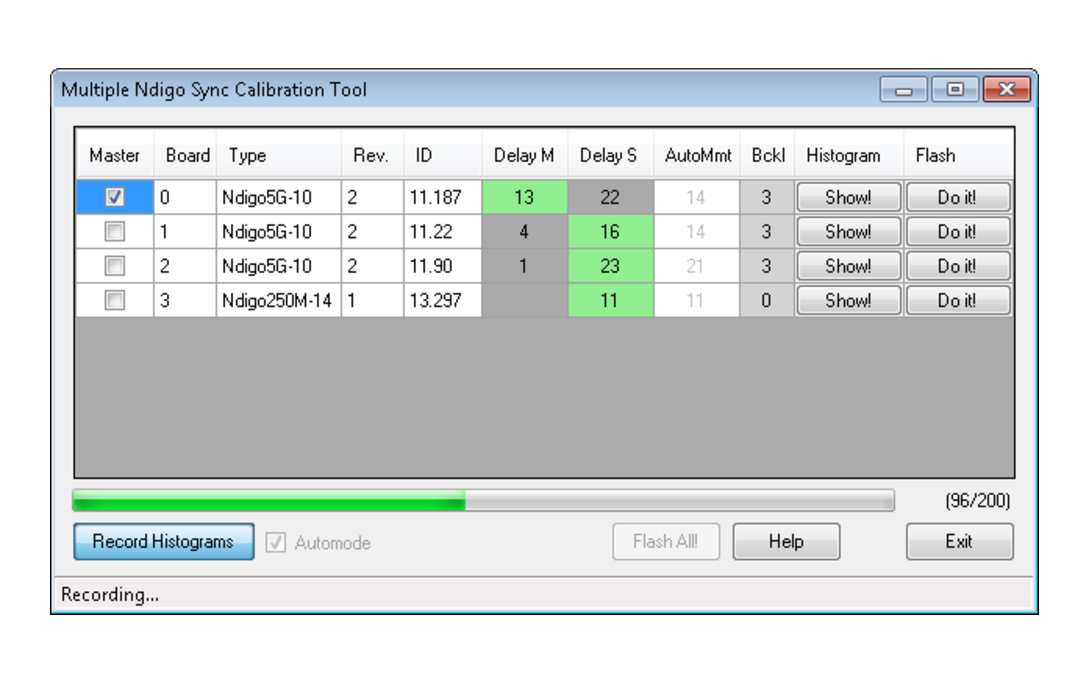
\includegraphics[width=0.7\textwidth]{figures/SyncCalibTool.pdf}
            \caption{Main window of the multiple boards sync calibration tool\label{fig:SyncCalibTool}}
        \end{center}
    \end{figure*}

    A board's appropriate delay depends on whether it operates in master or slave mode. The respective values can be set in the column ``Delay M'' (for master boards) and ``Delay S'' (for slave boards). The designated master board can be selected in the column ``Master''. The calibration procedure creates a histogram for each board displaying the current delay between the boards. The histogram can be viewed by clicking on ``Show!''. When the appropriate delay values are found they can be stored in the on-board flash PROM by clicking ``Do it!'' separately for each board. Clicking ``Flash All!'' will write the values to all boards at once. Please note: Flashing the values might take up to 10 seconds during which the program might not respond.\par

\textbf{Important note}: If the application reports a ``PLL not locked'' error check the cable. If the recording of histograms does not make progress check the cable. Make sure the cable is properly terminated at both ends and firmly attached to each card.

    \subsection{Calibration Procedure}

        \begin{enumerate}
            \item Make sure the ``Automode'' is selected.
            \item Record the calibration histograms by pressing ``Record histograms''. The program will perform up to 200 measurements of the sync delay. After accumulating some data, the delay values found are reported in the column ``AutoMmt''. The values can be verified by examining the histogram that was recorded. A board's histogram should look like the one shown in Figure \ref{fig:HistoUncalib}. During normal operation the delay will be adjusted such that the data points accumulated roughly coincide with the vertical markers in the upper panel. As the delay pattern is periodic valid delay values are between 0 and 31. Thus, the delay value found by the auto measurement should correspond to the distance between the vertical markers and accumulated data points. Hint: When moving the mouse pointer across the histogram the delay value of the current location is displayed.
            \item After stopping the data acquisition, by pressing ``Record Histograms'' again or waiting for 200 measurements to complete, the delay values of the auto measurement need to be copied to the columns ``Delay M'' or ``Delay S'' depending on the corresponding board being a master or a slave. The correct field to copy the value to is highlighted in green.
            \item You may record a new dataset as a crosscheck that the delay is now set to an appropriate value. By disabling ``Automode'' the new delay values are used. Press ``Record Histograms'' in order to start the data acquisition. After some time the histogram should look similar to the one in Figure \ref{fig:HistoCalib}.
            \item The delay values for all boards in a set needs to be found. For the case a board acts as a master, the value ``Delay M'' needs to be adjusted, in case it is a slave, the ``Delay S'' parameter needs to be changed. In order to find the master-case delay values for all boards, the calibration procedure needs to be performed with every board acting as a master once. After changing the master board, the slave values of the other boards don't need to be readjusted. Only Ndigo5G boards may be set as masters. Therefore, a Ndigo250M board only needs to be calibrated as a slave.
            \item After finding all delay values, write the values to the on-board flash PROMs by pressing ``Flash All!''.
        \end{enumerate}

        \begin{figure*}[ht]
            \begin{center}
                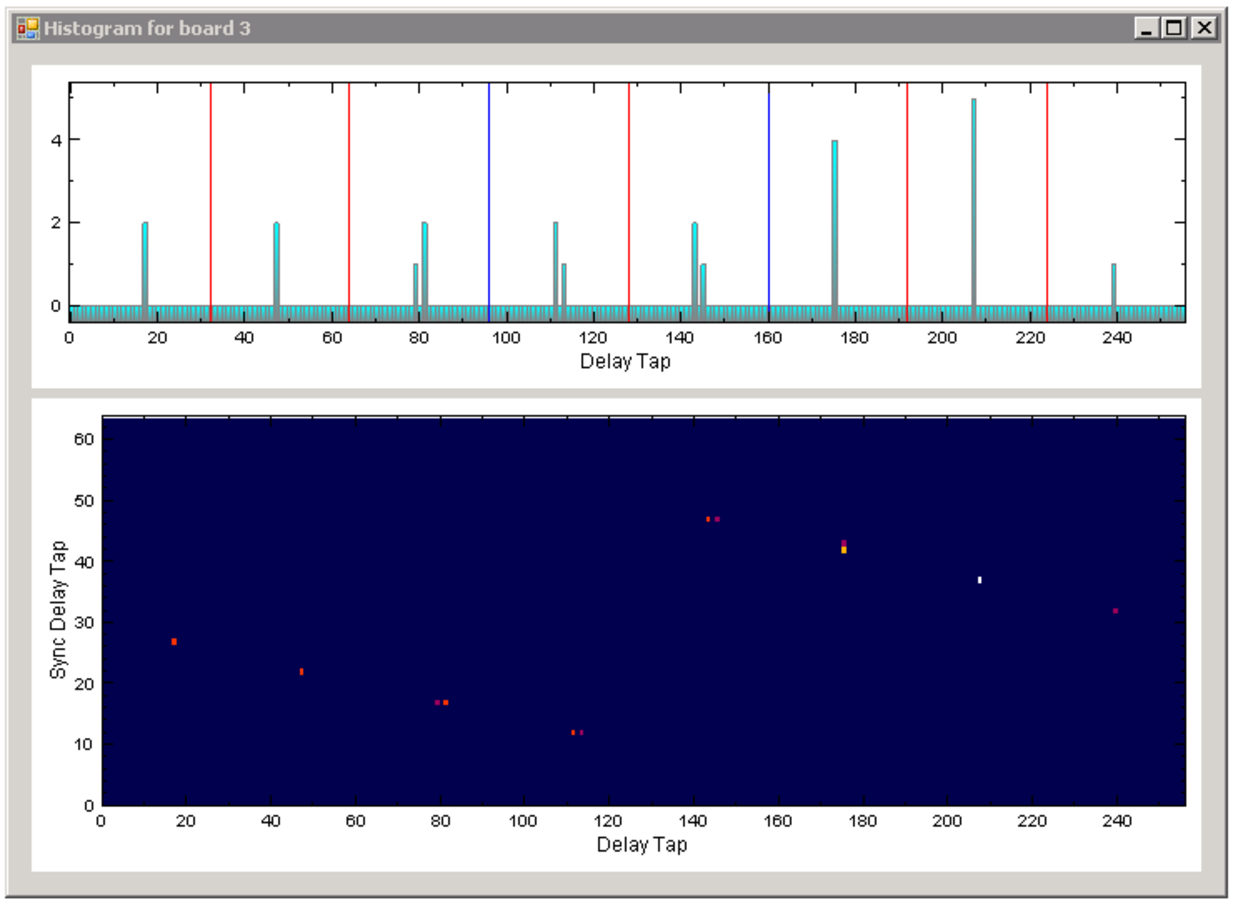
\includegraphics[width=0.6\textwidth]{figures/HistoUncalib.pdf}
                \caption{Histogram for the case the delay value for the board is not set correctly. Please note: the lower panel might differ from board to board, with the ``step'' being at a different position.\label{fig:HistoUncalib}}
            \end{center}
        \end{figure*}

        \begin{figure*}[hb]
            \begin{center}
                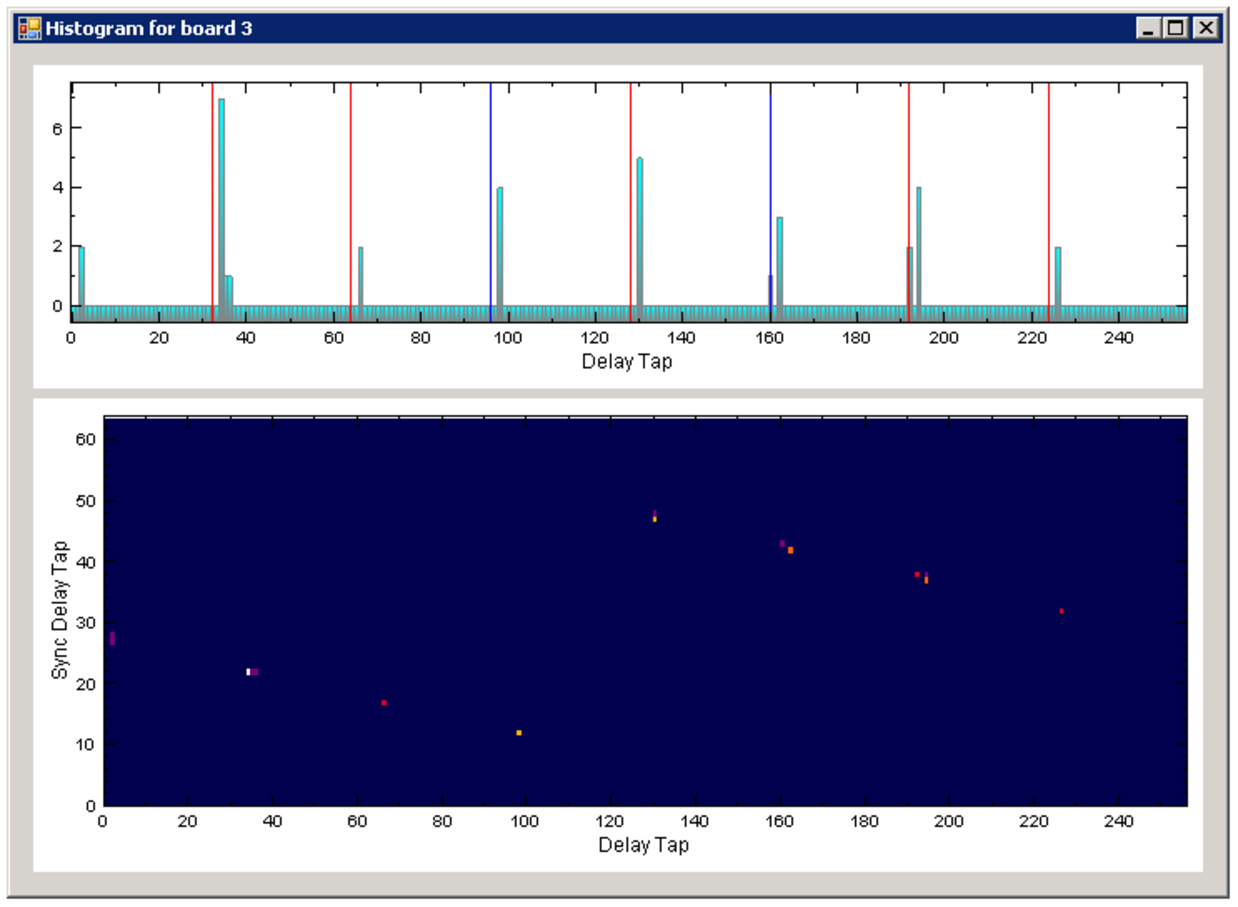
\includegraphics[width=0.6\textwidth]{figures/HistoCalib.pdf}
                \caption{Histogram for the case the delay value for the board is set correctly. Please note: the lower panel might differ from board to board, with the ``step'' being at a different position.\label{fig:HistoCalib}}
            \end{center}
        \end{figure*}

    \subsection{Synchronizing a Ndgio5G and an HPTDC8-PCI}

        In order to operate a Ndigo5G in sync with one or more HPTDC8-PCI boards, a board to board interconnection using a Ndigo Extension Board needs to be done. The Ndigo Extension Board has four clock outputs. One of them needs to be connected to the external clock input of the HPTDC using a standard LEMO00 cable. The Ndigo5G is connected to the Ndigo Extension Board using the Samtec ribbon cable provided with the Ndigo Extension Board. The signals used for synchronization of the boards are transmitted by a standard 10pin ribbon cable connecting the Ndigo Extension Board and the HPTDC. A schematic of all necessary connections is shown in Figure \ref{fig:InterconNdigo}.\par

        In principle the user can use the standard device drivers of the Ndigo5G and the HPTDC8-PCI to perform data acquisition. It is, however, recommended using the cronoSync library, which is a part of the cronoTools provided with the Ndigo5G device driver. cronoSync offers an easy group-based access to the data recorded and handles the synchronization of all cronologic data acquisition devices used. A detailed description of cronoTools and cronoSync can be found in the cronoTools user guide.

        \begin{figure*}[hb]
            \begin{center}
                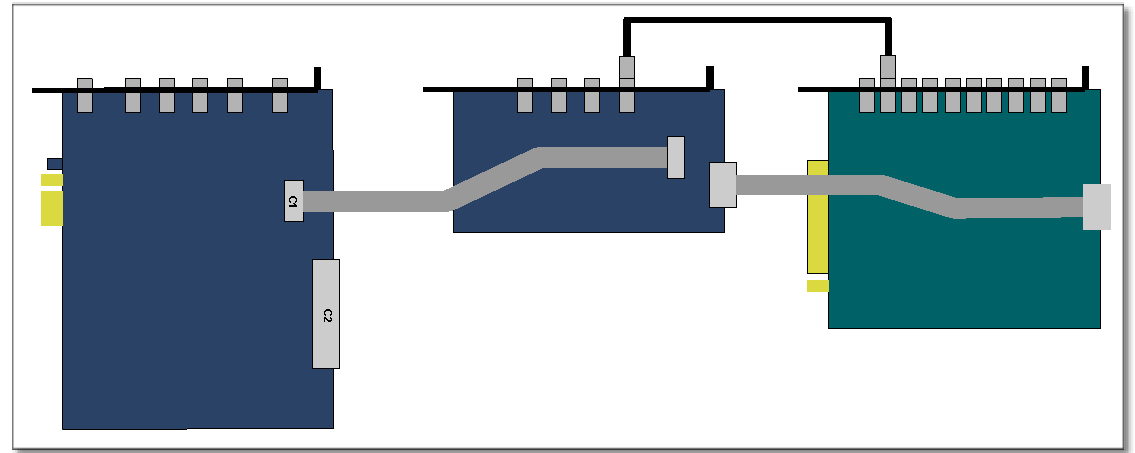
\includegraphics[width=\textwidth]{figures/InterconNdigo.pdf}
                \caption{\label{fig:InterconNdigo} Interconnection scheme of a Ndigo5G (left) and a HPTDC8-PCI (right) using a Ndigo Extension Board (middle).}
            \end{center}
        \end{figure*}

    \section{Performing a firmware update}

        After installing the Ndigo device driver, a firmware update tool is available, which is performed by choosing ``NdigoFirmwareGUI.exe''. After invoking the application a window as shown in Figure \ref{fig:Firmware} will appear. The tool can be used for updating the firmware and to create a backup of the on-board calibration data of the Ndigo unit. If several boards are present, the one which is going to be used can be selected in the upper left corner of the window. Pressing the ``Backup'' buttons a backup of the firmware or the calibration data will be created, respectively. In order to perform a firmware update, chose the ``.ndigorom''-file to used by pressing ``Browse''. The file contains the firmware PROMs for all boards of the Ndigo product line. By pressing ``Flash'' the firmware is written to the board. ``Verify'' can be used to compare the data stored inside the PROM to the one inside a file.\par

        \begin{figure*}[ht]
            \begin{center}
                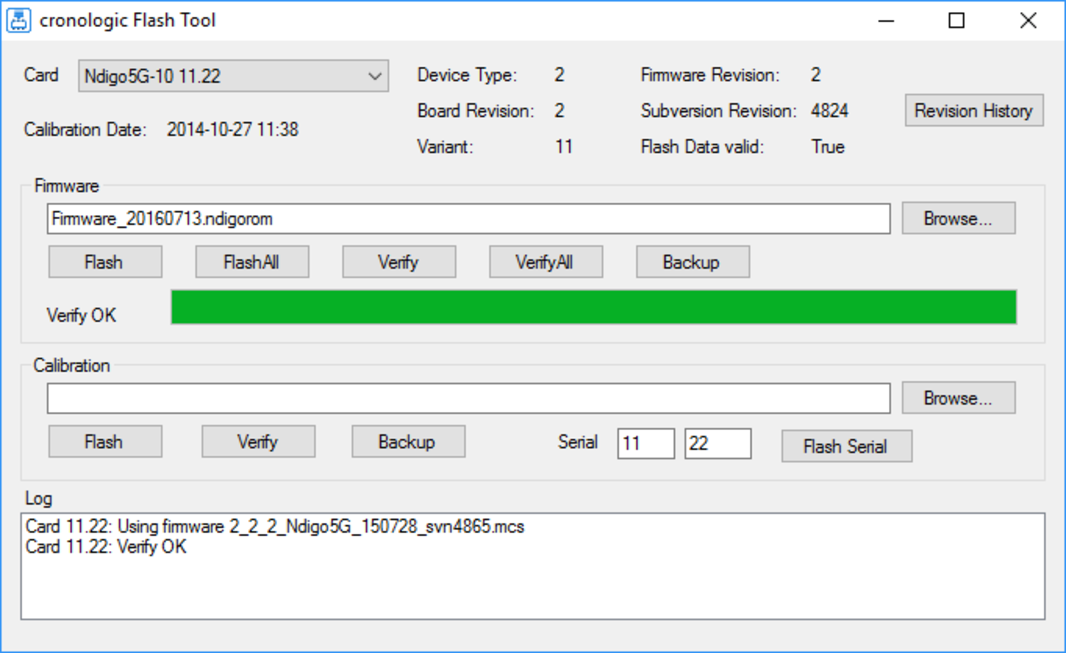
\includegraphics[width=0.8\textwidth]{figures/Firmware.pdf}
                \caption{\label{fig:Firmware}The firmware update and calibration data backup tool as provided with the Ndigo device driver.}
            \end{center}
        \end{figure*}

\textbf{Important note:} The new firmware will only be used after a power cycle, i.e. after switching the PC (or Ndigo crate) off and back on. \emph{A simple reboot is not sufficient.} Therefore, the information shown in the upper half of the application window does not change right after flashing a new firmware.\par
After flashing and shutting the PC or the crate off and on again it is recommended to perform a window calibration. The tool ``WindowCalibration'' is provided for that purpose within the driver installation. The omission of the calibration process leads to longer execution times of applications using that firmware, since the calibration is performed then instead.

    \section{Calibrating the TDC}

        After each update of the Ndigo5G-10 firmware the TDC has to be calibrated. The calibration is done with the tool ``TDC\tu Calibration.exe'' which is available after installing the Ndigo device driver. After invoking the application a window as shown in Figure \ref{fig:Calib} will appear.\par

        \begin{figure*}[ht]
            \begin{center}
                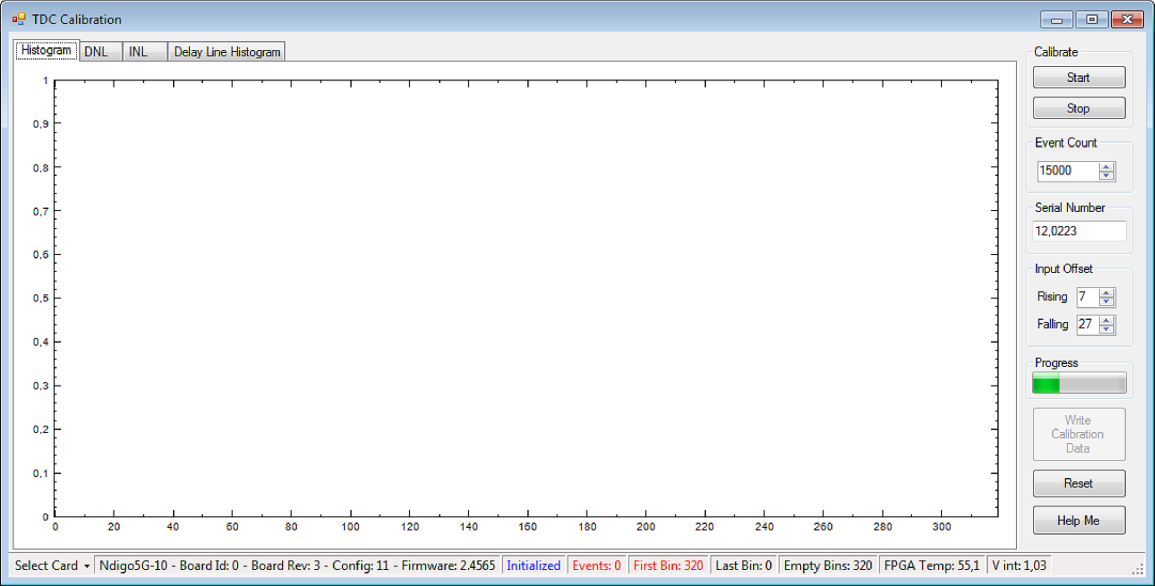
\includegraphics[width=0.8\textwidth]{figures/Calib.pdf}
                \caption{\label{fig:Calib}The TDC calibration tool as provided with the Ndigo device driver.}
            \end{center}
        \end{figure*}

        The calibration procedure is as follows:

        \begin{enumerate}
            \item Connect an external pulse signal to the Trigger input. The signal should be low active with a frequency in the kHz range. It must not be synchronized to the clock source of the Ndigo5G-10. The input frequency must not exceed 10 MHz. The pulse low and high width has to be at least 10ns each.
            \item Set \textit{Serial Number} according to the sticker on the card if the shown value is not correct.
            \item Start capturing pulse events by pressing the \textit{Start} button.
            \item Adjust the \textit{Input Offset} so that \textit{First Bin} is in the range of 4 to 16. If \textit{First Bin} is less than 4, increment \textit{Input Offset} by one. If \textit{First Bin} is greater than 16, decrement \textit{Input Offset} by one. Repeat increment/decrement until \textit{First Bin} is in the range of 4 to 16. Depending on the firmware revision the \textit{Input Offset} value for a successful calibration may be in the range of 6–10 or 28–32.
            \item When the \textit{Write Calibration Data} button becomes enabled press it to update the calibration data on the card.
            \item Calibration done!
        \end{enumerate}

        The card can only be successfully calibrated if:

        \begin{itemize}
            \item \textit{First Bin} is in the range of 4 to 16
            \item \textit{Empty Bins} is less than (First Bin + 4)
            \item at least 10,000 events have been captured
            \item a valid serial number is set.
        \end{itemize}

        \textbf{Important note:} If the application reports an error, check if the input pulse is within specification.
